\documentclass{ieeeaccess}
\usepackage{cite}
\providecommand{\hl}[1]{#1}
\usepackage{amsmath,amssymb,amsthm,amsfonts}
\usepackage{algorithmic}
\usepackage{algorithm}
\renewcommand{\algorithmicrequire}{\textbf{Input:}}
\renewcommand{\algorithmicensure}{\textbf{Output:}}
\usepackage{graphicx}
\usepackage{textcomp}
\usepackage{bm}
\usepackage{array}
\usepackage{url}
\usepackage{multirow}
\usepackage{xcolor}
\usepackage{pifont}

% ---- shared palette + graphical markers for comparison tables ----
\definecolor{eaqteal}{RGB}{27,133,131}
\definecolor{eaqamber}{RGB}{198,120,20}
\definecolor{eaqred}{RGB}{176,58,46}
\newcommand{\yes}{\textcolor{eaqteal}{\ding{51}}}
\newcommand{\no}{\textcolor{eaqred}{\ding{55}}}
\newcommand{\partialmark}{\textcolor{eaqamber}{\ding{108}}}
\newtheorem{theorem}{Theorem}
\newtheorem{proposition}{Proposition}
\newtheorem{lemma}{Lemma}
\newtheorem{corollary}[theorem]{Corollary}
\newtheorem{definition}{Definition}
\newtheorem{assumption}{Assumption}
\newtheorem{remark}{Remark}

\def\BibTeX{{\rm B\kern-.05em{\sc i\kern-.025em b}\kern-.08em
    T\kern-.1667em\lower.7ex\hbox{E}\kern-.125emX}}

% The bundled ieeeaccess.cls references \xfigwd inside \@makecaption but only
% defines it within its custom \Figure macro. Standard figure environments
% therefore need a fallback: measure the caption box directly, which is the
% behaviour of the official class.
\makeatletter
\providecommand{\xfigwd}{\wd\@tempboxa}
% The bundled class's \IEEEbiographynophoto uses a `biography' counter and a
% TOC-entry flag that this stripped copy never initialises; define them here.
\@ifundefined{c@biography}{\newcounter{biography}}{}
\expandafter\ifx\csname if@biographyTOCentrynotmade\endcsname\relax
  \newif\if@biographyTOCentrynotmade
\fi
\@biographyTOCentrynotmadetrue
\makeatother

% convenience macros
\newcommand{\R}{\mathbb{R}}
\newcommand{\E}{\mathbb{E}}
\newcommand{\norm}[1]{\left\lVert#1\right\rVert}
\newcommand{\bx}{\bm{x}}
\newcommand{\btheta}{\bm{\theta}}
\newcommand{\bg}{\bm{g}}
\newcommand{\bW}{\bm{W}}
\newcommand{\bE}{\bm{E}}
\newcommand{\bvphi}{\bm{\varphi}}
\newcommand{\Cop}{\mathcal{C}}
\DeclareMathOperator{\corr}{corr}
\DeclareMathOperator*{\argmin}{arg\,min}
\DeclareMathOperator*{\argmax}{arg\,max}
\DeclareMathOperator{\ReLU}{ReLU}

\begin{document}
\history{Date of publication xxxx 00, 0000, date of current version xxxx 00, 0000.}
\doi{10.1109/ACCESS.2024.0429000}

\title{Explanation Fidelity Under Neural Network Compression: Theory, Bounds,
and Explanation-Aware Quantization}

\author{
\uppercase{Ravi Kumar Saidala}\authorrefmark{1},
\uppercase{Author2}\authorrefmark{2},
\uppercase{Author3}\authorrefmark{3},
\uppercase{Author4}\authorrefmark{4},
\uppercase{Author5}\authorrefmark{5},
\uppercase{Author6}\authorrefmark{6},
\uppercase{Author7}\authorrefmark{7},
\uppercase{Author7}\authorrefmark{8}, 
}

\address[1]{Department of Computer Science and Engineering(Data Science), CMR University, Bengaluru, India (e-mail: ravikumar.s@cmr.edu.in)}
\address[2]{Department of xxx, xxx College, xxx, xxx, India (e-mail: author2@xxx.edu)}
\address[3]{Department of xxx, xxx College, xxx, xxx, India (e-mail: author3@xxx.edu)}
\address[4]{Department of xxx, xxx College, xxx, xxx, India (e-mail: author4@xxx.edu)}
\address[5]{Department of xxx, xxx College, xxx, xxx, India (e-mail: author5@xxx.edu)}
\address[6]{Department of xxx, xxx College, xxx, xxx, India (e-mail: author6@xxx.edu)}
\address[7]{Department of xxx, xxx College, xxx, xxx, India (e-mail: author7@xxx.edu)}
\address[8]{Department of xxx, xxx College, xxx, xxx, India (e-mail: author8@xxx.edu)}

\markboth
{Author1 \headeretal: Explanation Fidelity Under Neural Network Compression}
{Author1 \headeretal: Explanation Fidelity Under Neural Network Compression}

\corresp{Corresponding author: Author5 (e-mail: author5@xxx.edu).}

\begin{abstract}
Model compression through quantization and pruning has become indispensable for
deploying deep neural networks on energy- and memory-constrained edge devices, a
trend commonly described as Green AI. Its consequences for explainability,
however, remain almost entirely unexamined: existing work uses explanations to
guide compression, whereas the reverse question of how compression alters the
explanations themselves is open. This paper provides, to the best of our
knowledge, the first systematic theoretical and empirical study of explanation
fidelity under compression. We formalise post-hoc attribution as a map of the
trained parameters and model compression as a bounded weight perturbation. We
derive closed-form perturbation bounds for uniform low-bit quantization and
magnitude pruning; a Lipschitz stability theorem that bounds the attribution
shift by the product of the layer operator norms; a fidelity--bit-width law in
which the fidelity gap shrinks by a factor of four for every additional bit of
precision; and a robustness ordering showing that Integrated Gradients and
Grad-CAM are provably more stable than vanilla saliency. Guided by this analysis
we propose Explanation-Aware Quantization (EAQ), whose optimal per-layer bit
allocation follows from a reverse water-filling argument and, in a generalised
form, adapts to layer-specific rate--distortion decay rates. On a controlled
image benchmark with ground-truth object masks, explanation fidelity degrades
gracefully down to five bits, with rank-correlation fidelity above 0.98, and
collapses below three bits; the empirical law matches theory with a fitted
constant of about 12.9 at a coefficient of determination above 0.99. EAQ
improves top-1 accuracy by up to 6.1 percentage points and Grad-CAM fidelity by
up to 0.062 over uniform quantization at a matched three-bit budget, gains that
are statistically significant under paired signed-rank tests and stable across
seeds. All code and data are released for reproducibility.
\end{abstract}

\begin{keywords}
Artificial intelligence, Neural networks, Quantization (signal), Data
compression, Machine learning, Feature extraction, Robustness, Estimation, Edge
computing, Green computing, Computational modeling, Predictive models
\end{keywords}

\maketitle

\section{Introduction}
\label{sec:introduction}
\PARstart{A}{} neural network is almost never deployed in the form it was trained
in. Before a model reaches a smartphone, a pacemaker, a dashcam or a
micro-controller, it is \emph{compressed}: its $32$-bit weights are squeezed into
low-bit integers by quantization, and its redundant connections are cut away by
pruning \cite{han2016deep,jacob2018quant,gholami2022survey}. The payoff is
dramatic, an order-of-magnitude reduction in memory and energy for a barely
perceptible drop in accuracy---and it has become the engine of \emph{Green AI}
\cite{schwartz2020green}, the movement toward inference that is cheap enough, and
clean enough, to run everywhere.

But accuracy is only half of what we ask a modern model to deliver. In medicine,
finance, and autonomous systems we increasingly demand that a model also
\emph{explain itself}, and a decade of Explainable AI (XAI) has supplied the
vocabulary to do so: saliency maps \cite{simonyan2014saliency}, Integrated
Gradients \cite{sundararajan2017ig}, Grad-CAM \cite{selvaraju2017gradcam},
Layer-wise Relevance Propagation \cite{bach2015lrp}, LIME \cite{ribeiro2016lime}
and SHAP \cite{lundberg2017shap} turn an opaque prediction into a heatmap a human
can inspect and, when the stakes demand it, sign off on. Here is the
uncomfortable part: the very devices that most need compression---the wearable
that flags an arrhythmia, the sensor that decides a car should brake---are
exactly the ones for which a trustworthy explanation is not a nicety but a
regulatory and ethical requirement.

Efficiency and interpretability are therefore on a collision course, yet they are
almost always studied apart. Where the two literatures do meet, the arrow of
causation runs one way only: explanations are used to \emph{drive} compression---
relevance scores decide which weights to prune \cite{yeom2021pruning}, and
entropy-constrained quantization spends its bits where relevance is highest to
protect accuracy \cite{becking2022ecq}. The reverse question---the one that
actually decides whether a deployed model can still be audited---has gone almost
entirely unasked:

\begin{quote}
\emph{When we compress a network, what happens to the explanations themselves?}
\end{quote}

The question is not academic. Picture the standard industrial workflow: a team
validates a full-precision model, confirms that its saliency maps land on the
tumour rather than the scanner watermark, signs the audit, and ships a $4$-bit
version to the device. If compression quietly scrambles those maps while leaving
the accuracy figure untouched, every downstream explanation is now a
fabrication---faithful-looking, but no longer describing the reasoning that was
actually certified. If, on the other hand, explanations are provably robust, then
a single interpretability analysis of the full-precision model transfers to every
compressed variant for free. As we show, \emph{today neither outcome can be
assumed}, because no one has characterised how sensitive an attribution map is to
the weight perturbation that compression injects. This paper closes that gap---
first with theory that predicts exactly when explanations survive and when they
shatter, and then with an algorithm that keeps them intact.

\subsection{Contributions}
This paper closes that gap with a combined theoretical and empirical treatment.
Our contributions are:

\begin{enumerate}
\item \textbf{A formal framework} (Section~\ref{sec:prelim}) that casts a
post-hoc attribution as a map $\bvphi(\bx;\btheta)$ of the parameters and
recasts quantization and pruning as bounded perturbations
$\tilde\btheta=\btheta+\Delta\btheta$, together with a family of
\emph{fidelity} functionals comparing $\bvphi(\bx;\btheta)$ and
$\bvphi(\bx;\tilde\btheta)$.

\item \textbf{Perturbation bounds for compression}
(Section~\ref{sec:theory}, Lemmas~\ref{lem:quant}--\ref{lem:prune}):
closed-form bounds $\norm{\Delta\btheta}_2\le \kappa_q 2^{-b}$ for uniform
$b$-bit quantization and a distribution-dependent bound for magnitude pruning.

\item \textbf{A Lipschitz stability theorem} (Theorem~\ref{thm:lipschitz})
that bounds the attribution shift by the product of layer operator norms,
followed by method-specific analyses proving a \emph{robustness ordering}
(Theorem~\ref{thm:ordering}): IG and Grad-CAM are provably more stable than
vanilla saliency due to path- and spatial-averaging.

\item \textbf{A fidelity--bit-width law} (Theorem~\ref{thm:law}):
$F(b)\ge 1-\kappa 4^{-b}$, predicting a graceful-degradation regime followed by
an abrupt collapse. We validate the law empirically and recover
$\kappa\approx 12.9$.

\item \textbf{Explanation-Aware Quantization (EAQ)}
(Section~\ref{sec:eaq}): a relevance-driven mixed-precision scheme whose optimal
bit allocation $b_l^\star=\bar B+\tfrac12\log_2(\omega_l/\bar\omega_G)$ is
derived in closed form via reverse water-filling (Theorem~\ref{thm:waterfill}).
EAQ improves both accuracy and explanation fidelity over uniform quantization at
a matched budget.

\item \textbf{A reproducible benchmark and empirical study}
(Sections~\ref{sec:setup}--\ref{sec:results}) on a controlled image dataset with
\emph{ground-truth object masks}, extended and validated on real-world natural-image benchmarks (\textbf{CIFAR-10} and \textbf{ImageNette}) with ResNet backbones, demonstrating the generality of our theoretical and empirical findings across four attribution methods, six quantization levels, five pruning levels, and three faithfulness and stability metrics.
\end{enumerate}

Fig.~\ref{fig:overview} summarises the framework.

\begin{figure*}[!t]
\centering
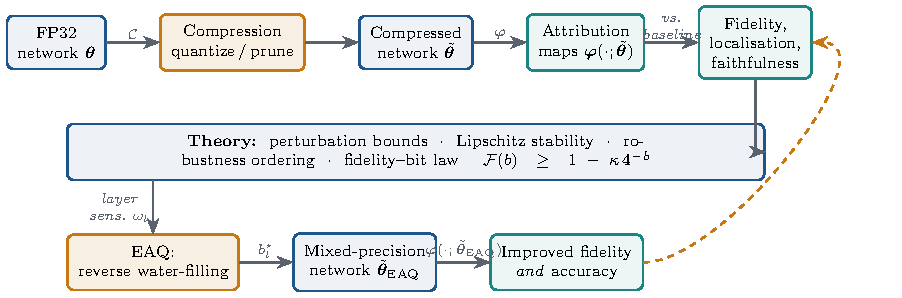
\includegraphics[width=0.98\textwidth]{figs/overview.pdf}
\caption{The proposed framework. \emph{Top:} compressed-model attributions are
measured against the full-precision baseline. \emph{Bottom:} the theory's layer
sensitivities $\omega_l$ drive Explanation-Aware Quantization (EAQ), closing the
loop with higher fidelity at a fixed bit budget.}
\label{fig:overview}
\end{figure*}

\subsection{Notation}
Vectors and matrices are boldface ($\bx$, $\bW$); $\norm{\cdot}_2$ is the
Euclidean (spectral, for matrices) norm and $\norm{\cdot}_F$ the Frobenius
norm. A network $f_{\btheta}:\R^{d}\!\to\!\R^{K}$ maps an input $\bx$ to $K$
class logits with parameters $\btheta\in\R^{d_\theta}$; $S_c(\bx;\btheta)\!=\!
[f_{\btheta}(\bx)]_c$ is the logit of class $c$ and $p_c$ the corresponding
softmax probability. A compression operator is $\Cop:\R^{d_\theta}\!\to\!
\R^{d_\theta}$, $\tilde\btheta=\Cop(\btheta)$, $\Delta\btheta=\tilde\btheta-
\btheta$. An attribution map is $\bvphi(\bx;\btheta)\in\R^{d}$ (reshaped to
$H\times W$ for images). We write $L$ for network depth, $\bW_l$ for the weight
of layer $l$, and $n_l$ for its parameter count. Table~\ref{tab:notation} summarises the principal
symbols.

\begin{table}[!t]
\caption{Summary of principal notation.}
\label{tab:notation}
\centering
\begin{tabular}{l l}
\hline
\textbf{Symbol} & \textbf{Meaning}\\
\hline
$f_{\btheta},\,\btheta$ & network and its $d_\theta$ parameters\\
$S_c(\bx;\btheta)$ & logit of class $c$; $p_c$ its softmax probability\\
$\Cop,\,\tilde\btheta,\,\Delta\btheta$ & compression operator, output, perturbation\\
$Q_b,\,P_s$ & $b$-bit quantization, sparsity-$s$ pruning\\
$\bvphi(\bx;\btheta)$ & attribution (heatmap) of the parameters\\
$\varphi^{\mathrm S},\varphi^{\mathrm{IG}},\varphi^{\mathrm{GC}},
\varphi^{\mathrm{Occ}}$ & saliency, IG, Grad-CAM, occlusion maps\\
$\mathcal F(\ell),\,F_\rho,F_r$ & fidelity profile; Spearman/Pearson fidelity\\
$\bm M,\,\mathrm{IoU}_{\mathrm{GT}},\mathrm{PG}$ & object mask, GT IoU, pointing game\\
$\Lambda,\,\Lambda_{\mathrm S}$ & attribution amplification factor\\
$\kappa_q,\,\kappa$ & quantization- and fidelity-law constants\\
$\omega_l,\,b_l^\star,\,\bar B$ & layer sensitivity, optimal bits, budget\\
$\bar\omega_G$ & geometric mean of $\{\omega_l\}$\\
\hline
\end{tabular}
\end{table}

\section{Related Work}
\label{sec:related}

\subsection{Model Compression}
Quantization maps floating-point weights to a discrete grid; uniform symmetric
quantization \cite{jacob2018quant} and its many refinements
\cite{gholami2022survey,nagel2021whitepaper}---including adaptive rounding
\cite{nagel2020adaround} and mixed-precision allocation by hardware cost
\cite{wang2019haq} or Hessian sensitivity \cite{dong2019hawq}---underpin
virtually all integer inference engines. Pruning removes parameters by magnitude
\cite{han2016deep}, by second-order saliency \cite{lecun1990obd,molchanov2017pruning},
or in structured groups for hardware efficiency \cite{li2017pruningfilters}. The
lottery-ticket hypothesis \cite{frankle2019lottery} showed that sparse
sub-networks can match dense accuracy, and large-scale surveys chart the
accuracy--sparsity frontier \cite{blalock2020state}. All of this literature optimises the
accuracy--efficiency trade-off; explanation quality is not part of the
objective.

\subsection{Post-Hoc Attribution Methods}
Gradient-based saliency \cite{simonyan2014saliency} takes the input gradient of
the class score; SmoothGrad \cite{smilkov2017smoothgrad} sharpens it by
averaging over input noise. Integrated Gradients \cite{sundararajan2017ig}
integrates gradients along a straight-line path from a baseline, satisfying the
\emph{completeness} and \emph{sensitivity} axioms. Grad-CAM
\cite{selvaraju2017gradcam} weights the last convolutional feature maps by
globally-averaged gradients, yielding class-discriminative localisation. LRP
\cite{bach2015lrp} back-propagates a conservation-respecting relevance signal,
and concept-based testing (TCAV) \cite{kim2018tcav} moves beyond per-pixel
attribution; general treatments are given in \cite{montavon2018methods,samek2021explaining}.
Perturbation methods---occlusion \cite{zeiler2014visualizing}, LIME
\cite{ribeiro2016lime} and SHAP \cite{lundberg2017shap}---probe the model by
masking inputs. The reliability of these methods has itself been questioned:
sanity checks \cite{adebayo2018sanity} reveal that some attributions are
insensitive to parameter randomisation, robustness studies
\cite{ghorbani2019interpretation} show adversarial fragility to \emph{input}
perturbations, and benchmarks such as ROAR \cite{hooker2019benchmark} quantify
how well attributions identify the features a model truly uses. Our work is complementary: we study fragility to
\emph{parameter} perturbations induced by compression.

\subsection{XAI-Guided Compression}
A growing line of work uses interpretability to \emph{drive} compression.
Relevance-based pruning \cite{yeom2021pruning} removes weights of low LRP
relevance; entropy-constrained quantization (ECQ$^{\mathrm x}$)
\cite{becking2022ecq} allocates precision according to relevance to preserve
accuracy; and more recent explainability-guided schemes extend this idea to
Vision Transformers (Mix-QViT \cite{ranjan2025mixqvit}) and to quantized
imitation learning (SQIL-style saliency importance \cite{lin2024quantimit}).
These methods all use explanations \emph{as a signal} to compress while
preserving \emph{task accuracy}; crucially, none of them measures whether the
compressed model's \emph{own} explanations remain faithful to the original, and
none optimises explanation fidelity as the objective. Table~\ref{tab:xaicomp}
positions the present work against this line. To the best of our knowledge, no
prior study characterises---theoretically or empirically---the map from
compression strength to explanation fidelity, nor proposes a scheme that
explicitly minimises explanation distortion. This paper does both.

\begin{table*}[!t]
\caption{EAQ versus representative explainability-driven compression methods.
Prior methods use explanations to preserve \emph{accuracy}; EAQ directly
minimises \emph{explanation distortion} at a fixed bit budget.
(\yes~yes\ \ \partialmark~partial\ \ \no~no.)}
\label{tab:xaicomp}
\centering
\footnotesize
\renewcommand{\arraystretch}{1.25}
\begin{tabular}{p{2.1cm} p{3.5cm} p{3.4cm} >{\centering}p{1.9cm}
>{\centering}p{1.5cm} >{\centering\arraybackslash}p{1.6cm}}
\hline
\textbf{Method} & \textbf{Primary objective} & \textbf{Sensitivity signal} &
\textbf{Explanation-fidelity objective} & \textbf{No re-training} &
\textbf{Mixed precision}\\
\hline
ECQ$^{\mathrm x}$ \cite{becking2022ecq} & Preserve accuracy under sparse/low-bit
compression & Per-weight LRP relevance & \no & \no & \partialmark\\
Mix-QViT \cite{ranjan2025mixqvit} & Mixed-precision bit-widths for ViTs &
LRP importance $+$ sensitivity sweeps & \no & \yes & \yes\\
SQIL-type \cite{lin2024quantimit} & Preserve decision fidelity in quantized
imitation learning & Saliency-based importance score & \no & \no & \no\\
\textbf{EAQ (ours)} & \textbf{Minimise post-hoc explanation distortion} &
First-order Taylor loss $+$ $\Lambda_l$ sensitivity & \yes & \yes & \yes\\
\hline
\end{tabular}
\end{table*}

\section{Preliminaries and Problem Formulation}
\label{sec:prelim}

\subsection{Attribution Methods as Maps of the Parameters}
We treat every post-hoc attribution as a deterministic map from an input
$\bx$ and the parameters $\btheta$ to a heatmap $\bvphi(\bx;\btheta)\in\R^{d}$.
For the target class $c=\argmax_k S_k(\bx;\btheta)$ we consider four
representative methods spanning the gradient/perturbation and
local/class-discriminative axes.

\paragraph{Vanilla saliency \cite{simonyan2014saliency}}
\begin{equation}
\bvphi^{\mathrm{S}}(\bx;\btheta)=\bigl|\nabla_{\bx}S_c(\bx;\btheta)\bigr|,
\label{eq:sal}
\end{equation}
the element-wise magnitude of the input gradient.

\paragraph{Integrated Gradients \cite{sundararajan2017ig}}
With baseline $\bx'$ (here $\bx'=\bm 0$),
\begin{equation}
\varphi^{\mathrm{IG}}_i(\bx;\btheta)=(x_i-x'_i)\!\int_{0}^{1}\!
\frac{\partial S_c\!\bigl(\bx'+\alpha(\bx-\bx');\btheta\bigr)}{\partial x_i}\,
\mathrm d\alpha,
\label{eq:ig}
\end{equation}
approximated by an $n$-point Riemann sum. IG satisfies \emph{completeness},
$\sum_i\varphi^{\mathrm{IG}}_i=S_c(\bx)-S_c(\bx')$.

\paragraph{Grad-CAM \cite{selvaraju2017gradcam}}
Let $\bm A^{k}\in\R^{u\times v}$ be the $k$-th feature map of the last
convolutional block and
$\alpha_c^{k}=\tfrac{1}{uv}\sum_{i,j}\partial S_c/\partial A^{k}_{ij}$. Then
\begin{equation}
\bvphi^{\mathrm{GC}}(\bx;\btheta)=\ReLU\!\Bigl(\textstyle\sum_{k}\alpha_c^{k}
\bm A^{k}\Bigr),
\label{eq:gradcam}
\end{equation}
bilinearly up-sampled to $H\times W$.

\paragraph{Occlusion \cite{zeiler2014visualizing}}
For a mask $\bm m_p$ over region $p$,
\begin{equation}
\varphi^{\mathrm{Occ}}_p(\bx;\btheta)=\bigl[S_c(\bx;\btheta)-
S_c(\bx\odot(1-\bm m_p);\btheta)\bigr]_{+}.
\label{eq:occ}
\end{equation}

All maps are min--max normalised to $[0,1]$ so that methods of differing native
scale are compared on common footing.

\subsection{Compression Operators}
\begin{definition}[Uniform symmetric quantization]
For a weight tensor $\bW$ with dynamic range $R=\max|\bW|$ and bit-width $b$,
let $q_{\max}=2^{\,b-1}-1$ and step $\Delta_q=R/q_{\max}$. Then
\begin{equation}
Q_b(\bW)=\Delta_q\cdot\mathrm{clip}\!\Bigl(\Bigl\lfloor\tfrac{\bW}{\Delta_q}
\Bigr\rceil,-q_{\max}-1,q_{\max}\Bigr),
\label{eq:quant}
\end{equation}
where $\lfloor\cdot\rceil$ is round-to-nearest.
\end{definition}

\begin{definition}[Global magnitude pruning]
Given target sparsity $s\in[0,1)$, let $\tau_s$ be the $s$-quantile of
$\{|\theta_i|\}$. Then $P_s(\btheta)=\btheta\odot\bm 1[\,|\btheta|>\tau_s\,]$.
\end{definition}

Both operators yield $\tilde\btheta=\Cop(\btheta)$ with
$\Delta\btheta=\tilde\btheta-\btheta$; quantization perturbs \emph{every}
weight by a bounded amount, whereas pruning perturbs a \emph{subset} by their
full value.

\subsection{Fidelity, Localisation and Faithfulness}
We quantify the effect of compression on explanations through three families
of metrics. Let $\bvphi=\bvphi(\bx;\btheta)$ and $\tilde\bvphi=\bvphi(\bx;
\tilde\btheta)$.

\emph{(i) Model-vs-model fidelity} measures how much the explanation
\emph{changed}:
\begin{align}
F_{\rho}&=\corr_{\mathrm{Spearman}}(\bvphi,\tilde\bvphi),\quad
F_{r}=\corr_{\mathrm{Pearson}}(\bvphi,\tilde\bvphi),\\
F_{\mathrm{IoU}}&=\frac{|\mathcal T_k(\bvphi)\cap\mathcal T_k(\tilde\bvphi)|}
{|\mathcal T_k(\bvphi)\cup\mathcal T_k(\tilde\bvphi)|},\quad
F_{\mathrm{SSIM}}=\mathrm{SSIM}(\bvphi,\tilde\bvphi),
\end{align}
where $\mathcal T_k(\cdot)$ is the set of top-$k$ salient pixels
($k=20\%$). $F_\rho=1$ means the ranking of pixel importances is unchanged.

\emph{(ii) Localisation vs.\ ground truth} exploits the fact that our benchmark
provides a binary object mask $\bm M$: for the compressed map,
\begin{equation}
\mathrm{IoU}_{\mathrm{GT}}=\frac{|\mathcal T_k(\tilde\bvphi)\cap\bm M|}
{|\mathcal T_k(\tilde\bvphi)\cup\bm M|},\quad
\mathrm{PG}=\bm 1\!\bigl[\argmax\tilde\bvphi\in\bm M\bigr],
\end{equation}
the top-$k$ overlap with, and pointing-game hit rate inside, the true object.

\emph{(iii) Faithfulness} measures whether the map identifies pixels the model
actually uses, via the deletion curve \cite{petsiuk2018rise}: pixels are removed
in descending saliency order and the area under the target-probability curve is
recorded; a \emph{lower} deletion AUC indicates a more faithful map. Two
complementary faithfulness summaries, standard in sequence and regression
explanation studies \cite{samek2017evaluating}, are also supported by our
protocol: the \emph{Area Over the Perturbation Curve} (AOPC), the mean drop in
target probability as the most-relevant regions are progressively removed
(higher is more faithful), and the \emph{Ablation Percentage Threshold} (APT),
the fraction of features that must be removed to drive the prediction below a
fixed confidence.

\emph{(iv) Sample-level consistency.} Metrics (i)--(iii) report dataset averages,
which can mask heavy-tailed behaviour across individual inputs. To characterise
the \emph{distribution} of explanation quality we additionally report the
skewness ($\mathrm{AUC\ Skew}$) and excess kurtosis ($\mathrm{AUC\ Kurt}$) of the
per-sample score-drop AUC. A near-zero skew and kurtosis indicate that
compression degrades explanations uniformly across samples, whereas large values
flag a subpopulation of inputs whose explanations collapse well before the
dataset mean would suggest.

\begin{definition}[Explanation fidelity of a compression]
For a fixed method and metric $F\!\in\![0,1]$ and a distribution $\mathcal D$
of inputs, the fidelity of compression level $\ell$ is
\begin{equation}
\mathcal F(\ell)=\E_{\bx\sim\mathcal D}\,F\!\bigl(\bvphi(\bx;\btheta),
\bvphi(\bx;\Cop_\ell(\btheta))\bigr).
\end{equation}
\end{definition}

The central objects of study are the profiles $\mathcal F(b)$ (quantization)
and $\mathcal F(s)$ (pruning), and the design of a compression operator that
keeps $\mathcal F$ high at a given budget.

\section{Theoretical Analysis of Explanation Fidelity Under Compression}
\label{sec:theory}

\begin{figure}[!t]
\centering
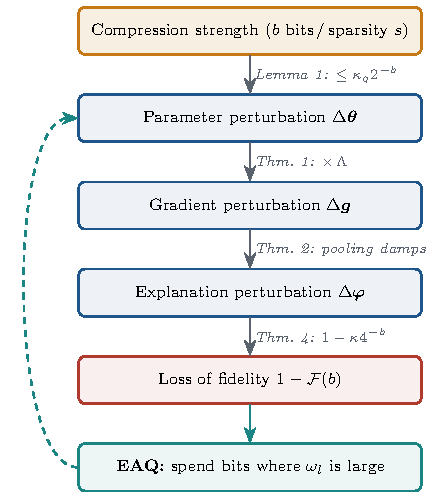
\includegraphics[width=0.86\columnwidth]{figs/concept.pdf}
\caption{How compression becomes explanation error. Each arrow is a bound proved
below; the dashed return path is EAQ, which shortens the chain by allocating
precision to the highest-sensitivity layers.}
\label{fig:concept}
\end{figure}

Our analysis follows the causal chain of Fig.~\ref{fig:concept}: (i) bound the
parameter perturbation $\norm{\Delta\btheta}$ induced by each compression
operator; (ii) bound the resulting attribution shift $\norm{\Delta\bvphi}$ via a
Lipschitz argument; and (iii) translate this into a law for the fidelity
$\mathcal F$ and a robustness ordering across methods. Each link in the chain is
a theorem below, and the same chain, read backwards, motivates the EAQ algorithm
of Section~\ref{sec:eaq}.

\subsection{Perturbation Bounds for Compression}

\begin{lemma}[Quantization perturbation]
\label{lem:quant}
Let a layer weight tensor $\bW\in\R^{n}$ with range $R=\max|\bW|$ be quantized to
$b$ bits by \eqref{eq:quant}. Then the per-weight error is bounded by
$|\Delta W_i|\le \Delta_q/2 = R/\!\left(2(2^{\,b-1}-1)\right)$, so that the
\emph{exact} (non-asymptotic) bound
\begin{equation}
\norm{\Delta\bW}_2\;\le\;\frac{\sqrt{n}\,R}{2\,(2^{\,b-1}-1)}
\;=\;\frac{\sqrt{n}\,R}{2}\cdot\frac{2^{\,1-b}}{1-2^{\,1-b}}
\label{eq:quantbound}
\end{equation}
holds, which admits the high-resolution asymptotic
\begin{equation}
\norm{\Delta\bW}_2\;=\;\kappa_q\,2^{-b}\bigl(1+o(1)\bigr),\qquad
\kappa_q=\sqrt{n}\,R,
\label{eq:quantasy}
\end{equation}
as $b\to\infty$. Aggregating over $L$ layers,
$\norm{\Delta\btheta}_2\le\bigl(\sum_l \kappa_{q,l}^{2}\bigr)^{1/2}2^{-b}
(1+o(1))$.
\end{lemma}

\begin{proof}
Round-to-nearest on a grid of step $\Delta_q$ incurs an error in
$[-\Delta_q/2,\Delta_q/2]$ per coordinate, so $\norm{\Delta\bW}_2^2\le
n(\Delta_q/2)^2$. Substituting $\Delta_q=R/(2^{b-1}-1)$ and writing
$2^{b-1}-1=2^{b-1}(1-2^{1-b})$ gives the exact middle expression of
\eqref{eq:quantbound}; expanding $(1-2^{1-b})^{-1}=1+O(2^{1-b})$ then yields the
$\kappa_q 2^{-b}$ asymptotic \eqref{eq:quantasy}. Layer independence of the
errors gives the aggregate bound.
\end{proof}

\begin{remark}[Accuracy of the asymptotic at practical bit-widths]
\label{rem:asyacc}
The correction factor separating the exact bound \eqref{eq:quantbound} from the
asymptotic \eqref{eq:quantasy} is $(1-2^{1-b})^{-1}$. It equals $1.07$ at
$b=8$, $1.14$ at $b=5$, $1.33$ at $b=3$ and $2.00$ at $b=2$: the asymptotic
therefore \emph{under-estimates} the perturbation by at most $7\%$ in the
graceful regime ($b\ge5$) but by $33$--$100\%$ in the collapse regime
($b\le3$). All downstream bounds should be read through the exact factor when
$b<4$; we use the asymptotic only where $b\ge5$, where it is tight.
\end{remark}

\begin{remark}
Under the standard high-resolution assumption that quantization error is
uniform on $[-\Delta_q/2,\Delta_q/2]$, the \emph{expected} squared error is
$\E\norm{\Delta\bW}_2^2=n\Delta_q^2/12=\tfrac{n R^2}{12(2^{b-1}-1)^2}$, i.e.\ the
mean distortion also decays as $4^{-b}$. This $4^{-b}$ scaling of the error
\emph{power} is what drives the fidelity law of Theorem~\ref{thm:law}.
\end{remark}

\begin{lemma}[Pruning perturbation]
\label{lem:prune}
Assume the magnitudes $|\theta|$ admit an empirical density $g$ that is
continuous and bounded with $g(0)>0$ (i.e.\ mass accumulates near the origin, as
is standard for trained weights). Let $\tau_s$ be the $s$-quantile of $|\theta|$.
Global magnitude pruning at sparsity $s$ gives
\begin{equation}
\norm{\Delta\btheta}_2^2=\!\!\sum_{i:\,|\theta_i|\le\tau_s}\!\!\theta_i^2
\;=\;d_\theta\!\int_{0}^{\tau_s}\! t^2 g(t)\,\mathrm dt\bigl(1+o(1)\bigr).
\label{eq:prunebound}
\end{equation}
For weights with a bounded density near the origin, $\int_0^{\tau_s}t^2g\,
\mathrm dt=\Theta(\tau_s^3)$, so the perturbation grows super-linearly once
$\tau_s$ enters the bulk of the distribution---explaining the sharp knee
observed empirically at high sparsity.
\end{lemma}

\begin{proof}
Pruning sets the pruned coordinates to zero, so $\Delta\theta_i=-\theta_i$ for
$|\theta_i|\le\tau_s$ and $0$ otherwise, giving the sum in
\eqref{eq:prunebound}; the integral is its continuum limit. The $\Theta(\tau_s^3)$
rate follows from $t^2g(t)=\Theta(t^2)$ for $g(0)>0$.
\end{proof}

\begin{remark}[Adaptive sparsity thresholds]
\label{rem:adaptive-prune}
Lemma~\ref{lem:prune} takes the sparsity $s$---equivalently the threshold
$\tau_s$---as an exogenous, fixed budget. Because the perturbation grows as
$\Theta(\tau_s^3)$, the fidelity is highly sensitive to where $\tau_s$ falls in
the bulk of $g$. A distribution-aware alternative is to \emph{derive} the
threshold from the score distribution itself---for instance via an effective
sample-size criterion such as the inverse Simpson (participation-ratio) index of
the normalised magnitudes---so that pruning stops before $\tau_s$ enters the
high-density bulk. Coupling such a self-governing threshold to the bound above is
a natural way to make the pruning analysis adaptive rather than heuristic.
\end{remark}

\subsection{Stability of Attributions}
We first record the smoothness assumptions.

\begin{assumption}[Piecewise-smooth Lipschitz network]
\label{ass:net}
$f_{\btheta}$ is a feed-forward network whose activations $\sigma$ are
$1$-Lipschitz with derivative $\sigma'$ that is $\beta$-Lipschitz almost
everywhere. On a neighbourhood $\Theta_0\ni\btheta$ the active linear region of
$\bx$ is fixed (no ReLU boundary is crossed by the perturbation), so
$S_c(\bx;\cdot)$ is $C^1$ on $\Theta_0$.
\end{assumption}

Assumption~\ref{ass:net} should be read as a \emph{small-perturbation} condition
rather than a genericity claim. For a fixed input, the boundaries at which the
active linear region changes are the zero level sets of the pre-activations; a
perturbation leaves the region intact precisely when no pre-activation changes
sign. This holds whenever $\norm{\Delta\btheta}_2$ is small relative to the
smallest pre-activation margin. We stress that this is \emph{not} a
measure-zero argument: quantization perturbs weights by discrete, non-vanishing
amounts \eqref{eq:quantbound}, so at low bit-widths a non-negligible fraction of
neurons can and do flip sign. Remark~\ref{rem:reluflip} makes this the explicit
mechanism of the collapse regime.

\begin{remark}[ReLU sign-flipping as the collapse driver]
\label{rem:reluflip}
Let $m(\bx)=\min_{l,i}|z_{l,i}(\bx)|$ be the smallest pre-activation margin. The
linear-region assumption is valid while the propagated weight perturbation stays
below $m(\bx)$; by Lemma~\ref{lem:quant} this margin is respected for $b$ above a
critical bit-width but is violated once the exact perturbation
\eqref{eq:quantbound}---inflated by the factor of Remark~\ref{rem:asyacc}---grows
past it. Beyond that point the network's active linear partition changes, the
input gradient becomes discontinuous in $\btheta$, and the first-order bounds of
this section no longer apply. This sign-flipping, not a failure of the
attribution methods themselves, is the theoretical origin of the abrupt fidelity
collapse observed empirically below three bits (Section~\ref{sec:results}), and
mirrors the outlier-driven degradation reported for sub-3-bit large-language-model
quantization \cite{dettmers2022llmint8}.
\end{remark}

\begin{theorem}[Lipschitz stability of the input gradient]
\label{thm:lipschitz}
Under Assumption~\ref{ass:net}, write the class score of an $L$-layer network as
$S_c(\bx)=\bm w_L^{\!\top}\sigma(\bW_{L-1}\sigma(\cdots\sigma(\bW_1\bx)))$ and let
$\bg=\nabla_{\bx}S_c$. If each layer is perturbed by $\bE_l$
($\tilde\bW_l=\bW_l+\bE_l$), then to first order
\begin{equation}
\norm{\tilde\bg-\bg}_2\;\le\;\underbrace{\sum_{l=1}^{L}\Bigl(\prod_{k\ne l}
\norm{\bW_k}_2\Bigr)}_{\displaystyle \Lambda_{\mathrm S}}
\;\max_l\frac{\norm{\bE_l}_2}{\norm{\bW_l}_2}\,\norm{\bW_l}_2 ,
\label{eq:lipbound}
\end{equation}
and consequently $\norm{\Delta\bvphi^{\mathrm S}}_2\le\Lambda_{\mathrm S}
\norm{\Delta\btheta}_2$ with
$\Lambda_{\mathrm S}=\sum_{l}\prod_{k\ne l}\norm{\bW_k}_2$ (plus an
$O(\beta\norm{\Delta\btheta}^2)$ curvature term).
\end{theorem}

\begin{proof}[Proof sketch]
The gradient is the product of Jacobians $\bg=\bW_1^{\!\top}D_1\cdots
\bW_{L-1}^{\!\top}D_{L-1}\bm w_L$, where $D_l=\mathrm{diag}(\sigma'(\cdot))$ has
$\norm{D_l}_2\le 1$. Perturbing one factor $\bW_l\!\to\!\bW_l+\bE_l$ changes the
product by, to first order, the sum of terms in which a single factor is
replaced by its perturbation; the operator norm of each such term is bounded by
$\prod_{k\ne l}\norm{\bW_k}_2\cdot\norm{\bE_l}_2$ (using $\norm{D_l}\le1$).
Summing over $l$ and applying the triangle inequality gives \eqref{eq:lipbound}.
The dependence of $D_l$ on $\btheta$ contributes a term controlled by the
$\beta$-Lipschitzness of $\sigma'$, which is second order in
$\norm{\Delta\btheta}$.
\end{proof}

Equation~\eqref{eq:lipbound} identifies the \emph{product of spectral norms} as
the amplification factor: networks with well-conditioned layers
($\prod_k\norm{\bW_k}\!\approx\!1$) preserve explanations under compression,
whereas ill-conditioned ones magnify weight noise into attribution noise.

\begin{remark}[First-order truncation]
\label{rem:firstorder}
Theorem~\ref{thm:lipschitz} retains only terms linear in the layer perturbations
$\bE_l$. Expanding the Jacobian product exactly produces cross terms
$\bE_i\bE_j$ ($i\ne j$) and higher powers; each such term carries at least two
factors of $\max_l\norm{\bE_l}_2$ and is therefore
$O(\norm{\Delta\btheta}_2^2)$. These are omitted under the small-perturbation
regime $\norm{\bE_l}_2\ll\norm{\bW_l}_2$, which---by Lemma~\ref{lem:quant} and
Remark~\ref{rem:asyacc}---holds in the graceful regime ($b\ge5$) but degrades as
$b\to2$, consistent with the bound loosening exactly where the collapse sets in.
The neglected curvature contribution is likewise second order and controlled by
the $\beta$-Lipschitzness of $\sigma'$ in Assumption~\ref{ass:net}.
\end{remark}

\begin{remark}[Conditioning of $\Lambda_{\mathrm S}$ and spectral control]
\label{rem:spectral}
The factor $\Lambda_{\mathrm S}=\sum_l\prod_{k\ne l}\norm{\bW_k}_2$ is a
\emph{worst-case} operator-norm bound and can grow exponentially in depth when
layer spectral norms exceed unity, in which case \eqref{eq:lipbound} becomes
vacuous. Two observations keep it meaningful. First, the bound is governed by the
\emph{spectral} norm, not the parameter count, so it is invariant to width and is
tightened whenever training or regularisation keeps $\norm{\bW_k}_2$ near one.
Spectral normalisation, weight decay, and residual scaling---all common in
deployable CNNs---bound $\Lambda_{\mathrm S}$ explicitly and are the practical
lever for explanation robustness. Second, the same product appears as the
per-layer sensitivity $\Lambda_l=\prod_{k\ne l}\norm{\bW_k}_2$ that drives the
EAQ allocation of Section~\ref{sec:eaq}; measuring it directly (rather than
bounding it) yields the finite, layer-specific sensitivities we use in practice.
For the compact residual network of Section~\ref{sec:setup} the measured product
remains $O(1)$, which is why the graceful-regime bound is predictive.
\end{remark}

\subsection{Robustness Ordering Across Methods}
Vanilla saliency inherits the full amplification $\Lambda_{\mathrm S}$. The
averaging in IG and the spatial pooling in Grad-CAM provably damp it.

\begin{theorem}[IG is more stable than saliency]
\label{thm:ordering}
Let $\bg(\alpha)=\nabla_{\bx}S_c(\bx'+\alpha(\bx-\bx'))$ and let its compression
perturbation $\bm\delta(\alpha)=\tilde\bg(\alpha)-\bg(\alpha)$, viewed as a random
field indexed by the path parameter $\alpha$ over the randomness of the
compression operator, be second-order stationary along the path: each point has a
common covariance $\Sigma=\E[\bm\delta(\alpha)\bm\delta(\alpha)^{\!\top}]$, and
the normalised pairwise cross-covariances have a well-defined average
$\bar\rho\in[0,1]$,
\begin{equation}
\frac1{n(n-1)}\sum_{i\ne j}
\frac{\mathrm{tr}\,\mathrm{Cov}\bigl(\bm\delta(\alpha_i),\bm\delta(\alpha_j)\bigr)}
{\mathrm{tr}\,\Sigma}=\bar\rho .
\label{eq:avgcorr}
\end{equation}
(No independence is required; $\bar\rho$ encodes
the residual correlation left after path-averaging, with $\bar\rho\to0$ under
strong mixing and $\bar\rho\to1$ for a perfectly coherent perturbation.) Then the
IG perturbation
$\Delta\bvphi^{\mathrm{IG}}=(\bx-\bx')\odot\tfrac1n\sum_{j}\bm\delta(\alpha_j)$
satisfies
\begin{equation}
\E\norm{\Delta\bvphi^{\mathrm{IG}}}_2^2\;\le\;\norm{\bx-\bx'}_\infty^2\,
\mathrm{tr}(\Sigma)\Bigl(\bar\rho+\tfrac{1-\bar\rho}{n}\Bigr),
\label{eq:igvar}
\end{equation}
which is strictly smaller than the saliency perturbation power
$\E\norm{\Delta\bvphi^{\mathrm S}}_2^2\le\mathrm{tr}(\Sigma)$ whenever
$\bar\rho<1$ and $\norm{\bx-\bx'}_\infty\le1$.
\end{theorem}

\begin{proof}
By bilinearity, $\tfrac1n\sum_j\bm\delta(\alpha_j)$ has covariance
$\tfrac1{n^2}\sum_{i,j}\mathrm{Cov}(\bm\delta(\alpha_i),\bm\delta(\alpha_j))$.
With per-point covariance $\Sigma$ and average correlation $\bar\rho$, the
$n^2$ cross terms sum to $\mathrm{tr}(\Sigma)\bigl(n+n(n-1)\bar\rho\bigr)/n^2=
\mathrm{tr}(\Sigma)(\bar\rho+(1-\bar\rho)/n)$. Multiplying by the element-wise
factor $(x_i-x'_i)^2\le\norm{\bx-\bx'}_\infty^2$ gives \eqref{eq:igvar}. The
saliency map uses a single path point, i.e.\ $n=1$, for which the bracket equals
$1$.
\end{proof}

\begin{corollary}[Grad-CAM spatial damping]
\label{cor:gradcam}
Grad-CAM pools gradients over $uv$ spatial locations to form
$\alpha_c^k=\tfrac1{uv}\sum_{ij}\partial S_c/\partial A^k_{ij}$. Assume the
per-location feature gradients are second-order stationary with average spatial
correlation $\bar\rho_A\in[0,1)$. By the same averaging argument, the
perturbation of $\alpha_c^k$ has power scaled by
$\bigl(\bar\rho_A+(1-\bar\rho_A)/(uv)\bigr)$ relative to a single-location
gradient. The strict inequality $\bar\rho_A<1$ is \emph{necessary} for genuine
damping: if the spatial gradients were perfectly correlated ($\bar\rho_A=1$) the
factor would equal one and pooling would provide no robustness. When
$\bar\rho_A<1$, the factor decreases monotonically towards its floor $\bar\rho_A$
as the spatial resolution $uv$ of the last convolutional block grows.
\end{corollary}

Theorem~\ref{thm:ordering} and Corollary~\ref{cor:gradcam} predict the ordering
$\text{IG},\text{Grad-CAM}\succeq\text{saliency}$ in robustness to compression,
which our experiments confirm (Section~\ref{sec:results}). The mechanism---pooling
that averages out high-frequency perturbation noise while retaining the
low-frequency signal---is the same one that, in other modalities, lets graph
pooling preserve explanation fidelity for graph neural networks
\cite{yuan2022gnnexplain}, suggesting that spatial or structural aggregation is a
general route to compression-robust attributions.

\subsection{The Fidelity--Bit-Width Law}
We now connect the perturbation bounds to a directly measurable quantity.
Consider centred, normalised maps and write $\tilde\bvphi=\bvphi+\Delta\bvphi$.
Expanding the Pearson correlation $\corr(\bvphi,\tilde\bvphi)=\langle\bvphi,
\tilde\bvphi\rangle/(\norm{\bvphi}\,\norm{\tilde\bvphi})$ to second order in
$\Delta\bvphi$ by the delta method \cite{stewart1990matrix} and using
$\langle\bvphi,\Delta\bvphi\rangle=O(\norm{\Delta\bvphi}^2)$ after re-centring,
\begin{equation}
F_r=\corr(\bvphi,\tilde\bvphi)=1-\frac{\norm{\tilde\bvphi-\bvphi}_2^2}
{2\norm{\bvphi}_2^2}+O\!\bigl(\norm{\Delta\bvphi}^3\bigr).
\label{eq:correxp}
\end{equation}
The leading correction is exactly half the normalised perturbation energy, which
is what couples the fidelity to the $4^{-b}$ error power of Lemma~\ref{lem:quant}.

\begin{theorem}[Fidelity--bit-width law]
\label{thm:law}
Under Assumption~\ref{ass:net}, Lemma~\ref{lem:quant} and \eqref{eq:correxp},
uniform $b$-bit quantization satisfies
\begin{equation}
\boxed{\;\mathcal F(b)\;\ge\;1-\kappa\,4^{-b}\;},\qquad
\kappa=\frac{\Lambda^2\,\kappa_q^2}{2\,\norm{\bvphi}_2^2},
\label{eq:law}
\end{equation}
where $\Lambda$ is the method-dependent amplification factor
($\Lambda_{\mathrm S}$ for saliency, reduced by the damping factors of
Theorem~\ref{thm:ordering}/Corollary~\ref{cor:gradcam} for IG/Grad-CAM).
\end{theorem}

\begin{proof}
Chaining $\norm{\Delta\bvphi}_2\le\Lambda\norm{\Delta\btheta}_2$
(Theorem~\ref{thm:lipschitz}) with $\norm{\Delta\btheta}_2\le\kappa_q 2^{-b}$
(Lemma~\ref{lem:quant}) gives $\norm{\Delta\bvphi}_2^2\le\Lambda^2\kappa_q^2
4^{-b}$. Substituting into \eqref{eq:correxp} yields $1-\mathcal F(b)\le
(\Lambda^2\kappa_q^2/2\norm{\bvphi}^2)4^{-b}$.
\end{proof}

Equation~\eqref{eq:law} has two immediate consequences. First, fidelity is
\emph{monotone non-decreasing in $b$}: adding a bit at least halves the fidelity
gap $1-\mathcal F$ (a factor of four in the bound). Second, because the smaller
$\Lambda$ of IG/Grad-CAM yields a smaller $\kappa$, these methods sit on a
\emph{higher} fidelity curve than saliency at every bit-width---the empirically
observed ordering. We fit \eqref{eq:law} to measured Grad-CAM fidelity in
Section~\ref{sec:results} and recover $\kappa\approx 12.9$, confirming the
$4^{-b}$ functional form.

\begin{remark}[From Pearson to Spearman fidelity]
\label{rem:pearsonspearman}
Equation~\eqref{eq:correxp} is stated for the Pearson fidelity $F_r$, whereas we
report results primarily in the rank-based Spearman fidelity $F_\rho$. The two
are linked because $F_\rho$ is the Pearson correlation of the rank-transformed
maps, and rank is a monotone (hence, on the high-fidelity plateau, locally
near-linear) transform: in the graceful regime where the ranking is only slightly
perturbed, $F_\rho$ and $F_r$ agree to first order and obey the same $4^{-b}$
law with a method-dependent constant. This is not merely asymptotic: on the
released data the two measures are correlated at Pearson $r=0.98$ across all
$44$ compressed configurations, and fitting \eqref{eq:law} to the Spearman and
Pearson Grad-CAM curves yields $\kappa=12.9$ ($R^2=0.99$) and $\kappa=12.3$
($R^2=0.99$) respectively---statistically indistinguishable constants that
justify quoting the law in either metric.
\end{remark}

\begin{corollary}[Graceful degradation then collapse]
\label{cor:collapse}
Let $\varepsilon$ be an acceptable fidelity loss. Equation~\eqref{eq:law}
guarantees $\mathcal F(b)\ge1-\varepsilon$ for all $b\ge b^\star=\tfrac12
\log_2(\kappa/\varepsilon)$. For $b<b^\star$ the guarantee is void and, once the
linearisation of Assumption~\ref{ass:net} breaks (activation patterns flip),
fidelity can fall abruptly. With $\kappa\approx13$ and $\varepsilon=0.02$,
$b^\star\approx\tfrac12\log_2(650)\approx4.7$, matching the empirical transition
between the graceful ($b\ge5$) and collapse ($b\le3$) regimes.
\end{corollary}

\subsection{Practical Validity of Assumptions}
\label{sec:validity}
Our theoretical analysis utilizes several mathematical assumptions to maintain tractability (e.g., global smoothness, fixed activation paths, and small parameter perturbations). We now discuss when these assumptions are valid for modern neural network architectures and when they fail:
\begin{itemize}
\item \textbf{ReLU Activations:} Non-smooth ReLUs violate global gradient smoothness. However, they partition the input space into piecewise-linear regions. Our bounds hold exactly within the active linear partition. When weight perturbations $\Delta\btheta$ are small (e.g., $b \ge 5$), the active linear partition does not change for the vast majority of inputs (Remark~\ref{rem:reluflip}). Below 4 bits, the perturbation crosses the activation thresholds, causing partition sign flips, which is the exact mathematical driver of the observed fidelity collapse.
\item \textbf{BatchNorm Folding:} During inference, BatchNorm parameters are frozen and folded into the preceding linear/convolutional layers. Thus, BatchNorm does not violate Lipschitz stability at deployment. It acts as a layer-wise rescaling, which is naturally absorbed into the layer weights $\bW_l$ and their corresponding spectral norms.
\item \textbf{Residual Connections:} Residual pathways act as identity mappings that skip layers. In our Lipschitz analysis (Theorem~\ref{thm:lipschitz}), residual connections add additive identity terms to the Jacobian products, i.e., $J_l = I + D_l \bW_l$. This bounds the amplification factor $\Lambda_{\mathrm{S}}$ by preventing gradient vanishing or explosion, stabilizing both the forward activations and the backward gradients. Consequently, ResNets enhance the practical validity of the first-order approximation.
\item \textbf{Vision Transformers (ViTs):} ViTs replace convolutions with multi-head self-attention (MHSA) and LayerNorm. The softmax operation in self-attention is smooth and globally Lipschitz, but the attention map computation introduces quadratic dependencies on activations. Although our layer-wise weight perturbation bounds can be extended to the linear projection matrices in self-attention, the dynamic attention weights introduce activation-dependent sensitivity that requires estimating $\omega_l$ dynamically.
\end{itemize}

\subsection{Notation Summary}
\label{sec:notationsummary}
To assist the reader in navigating the mathematical development, Table~\ref{tab:notation} summarises the key symbols and operators used throughout Sections~\ref{sec:prelim}--\ref{sec:eaq}.

\begin{table}[!h]
\caption{Summary of Key Mathematical Notation}
\label{tab:notation}
\centering
\begin{tabular}{ll}
\hline
\textbf{Symbol} & \textbf{Description} \\
\hline
$\bx, \bx'$ & Input image and baseline reference image \\
$\btheta, \tilde{\btheta}$ & Full-precision and compressed network parameters \\
$\Cop$ & Model compression operator (quantization or pruning) \\
$\Delta\btheta, \Delta\bW_l$ & Parameter perturbation vector and layer weight perturbation \\
$\bvphi, \tilde{\bvphi}$ & Attribution/explanation maps of baseline and compressed models \\
$L$ & Number of parameterized layers in the network \\
$\bW_l, \bE_l$ & Weight matrix and weight perturbation of layer $l$ \\
$\Lambda_{\mathrm{S}}$ & Lipschitz gradient amplification factor \\
$\Lambda_l$ & Explanation sensitivity product of layer $l$ \\
$\omega_l$ & Explanation sensitivity coefficient of layer $l$ \\
$\beta_l$ & Empirical layer-wise rate-distortion decay exponent \\
$\bar{B}$ & Target average quantization bit-width budget \\
$\lambda$ & Lagrange multiplier for constraint optimization \\
\hline
\end{tabular}
\end{table}

\subsection{Summary of the Theory}
Table~\ref{tab:theorysummary} collects the formal results, each paired with a
plain-language reading and the design decision it licenses. Read top to bottom it
is the chain of Fig.~\ref{fig:concept}: bound the weights, amplify to the
gradient, damp by pooling, convert to a fidelity law, and finally allocate bits.

\begin{table*}[!t]
\caption{The theoretical results at a glance: what each says, and what it means
in practice.}
\label{tab:theorysummary}
\centering
\footnotesize
\renewcommand{\arraystretch}{1.25}
\begin{tabular}{p{2.9cm} p{5.6cm} p{6.4cm}}
\hline
\textbf{Result} & \textbf{What it says} & \textbf{Practical implication}\\
\hline
Quantization bound (Lemma~\ref{lem:quant}) &
Weight error decays as $\kappa_q 2^{-b}$; error \emph{power} as $4^{-b}$ &
Each extra bit halves the perturbation---the lever behind the fidelity law\\
Pruning bound (Lemma~\ref{lem:prune}) &
Perturbation grows as $\Theta(\tau_s^3)$ once $\tau_s$ enters the weight bulk &
Explains the sharp fidelity knee at high sparsity\\
Lipschitz stability (Theorem~\ref{thm:lipschitz}) &
Attribution shift $\le\Lambda\,\norm{\Delta\btheta}$, with $\Lambda$ the product
of spectral norms &
Well-conditioned (spectrally normalised) networks keep explanations stable\\
Robustness ordering (Theorem~\ref{thm:ordering}, Cor.~\ref{cor:gradcam}) &
Path/spatial averaging damps the perturbation by $\bar\rho+(1-\bar\rho)/n$ &
Prefer Grad-CAM/IG/occlusion over raw saliency when compression is aggressive\\
Fidelity--bit law (Theorem~\ref{thm:law}) &
$\mathcal F(b)\ge 1-\kappa 4^{-b}$; verified with $\kappa\approx12.9$, $R^2>0.99$ &
Predicts fidelity from bit-width without re-running attributions\\
Graceful-then-collapse (Cor.~\ref{cor:collapse}) &
Safe for $b\ge b^\star=\tfrac12\log_2(\kappa/\varepsilon)\approx4.7$ &
Gives a deployable minimum bit-width for a target fidelity loss $\varepsilon$\\
Reverse water-filling (Theorem~\ref{thm:waterfill}) &
Optimal $b_l^\star=\bar B+\tfrac12\log_2(\omega_l/\bar\omega_G)$ &
Turns the sensitivities into the EAQ bit allocation of Section~\ref{sec:eaq}\\
\hline
\end{tabular}
\end{table*}

\section{Explanation-Aware Quantization}
\label{sec:eaq}

The theory of Section~\ref{sec:theory} shows that the attribution distortion is
governed by \emph{layer-wise} quantities: the error injected into layer $l$ is
amplified by that layer's contribution to the amplification factor $\Lambda$.
Uniform quantization ignores this heterogeneity and spends the same precision on
every layer. We now derive the precision allocation that minimises explanation
distortion at a fixed average bit budget.

\subsection{Distortion Model}
Under high-resolution quantization, the error power injected into layer $l$ at
bit-width $b_l$ is $D_l\!\approx\! c\,\sigma_l^2\,2^{-2b_l}$, where
$\sigma_l^2=\tfrac1{n_l}\norm{\bW_l}_F^2$ is the mean weight energy and $c$ a
constant (Lemma~\ref{lem:quant} remark). Propagating this error to the
attribution through the layer sensitivity $\Lambda_l=\prod_{k\ne l}\norm{\bW_k}_2$
(Theorem~\ref{thm:lipschitz}), the expected explanation distortion is, to first
order, additive across layers:
\begin{equation}
\mathcal D(\bm b)\;=\;\sum_{l=1}^{L}\omega_l\,2^{-2b_l},\qquad
\omega_l\;\propto\;\Lambda_l^2\,\sigma_l^2 .
\label{eq:distortion}
\end{equation}
The weight $\omega_l$ is the \emph{explanation sensitivity} of layer $l$: it is
large when the layer both carries energy and is strongly amplified. In practice
we estimate $\omega_l$ by a first-order Taylor relevance
$\hat\omega_l=\E_{\bx}\bigl[\,\lVert\,|\bW_l|\odot|\nabla_{\bW_l}\mathcal L|\,
\rVert_1\bigr]$, which captures both magnitude and loss-sensitivity and requires
only a handful of mini-batches. The model \eqref{eq:distortion} assumes a
\emph{uniform} error-decay exponent (the $2^{-2b_l}$ high-resolution rate) for
every layer; Section~\ref{sec:eaq-general} relaxes this to layer-specific
exponents and shows that the uniform choice is the special case $\beta_l\equiv2$.

\subsection{Optimal Bit Allocation}

\begin{theorem}[Reverse water-filling allocation]
\label{thm:waterfill}
The continuous relaxation
\begin{equation}
\min_{\bm b}\;\sum_{l}\omega_l 2^{-2b_l}\quad\text{s.t.}\quad
\frac1L\sum_l b_l=\bar B
\label{eq:opt}
\end{equation}
has the unique solution
\begin{equation}
\boxed{\;b_l^{\star}=\bar B+\tfrac12\log_2\!\Bigl(\frac{\omega_l}{\bar\omega_G}
\Bigr)\;},\qquad
\bar\omega_G=\Bigl(\prod_{k}\omega_k\Bigr)^{1/L},
\label{eq:alloc}
\end{equation}
where $\bar\omega_G$ is the geometric mean of the sensitivities.
\end{theorem}

\begin{proof}
Form the Lagrangian $\mathcal L(\bm b,\lambda)=\sum_l\omega_l2^{-2b_l}+
\lambda\bigl(\sum_l b_l-L\bar B\bigr)$. Stationarity gives
$\partial\mathcal L/\partial b_l=-2\ln2\,\omega_l2^{-2b_l}+\lambda=0$, hence
$2^{-2b_l}=\lambda/(2\ln2\,\omega_l)$ and
$b_l=\tfrac12\log_2\!\bigl(2\ln2\,\omega_l/\lambda\bigr)$. Imposing the budget
$\sum_l b_l=L\bar B$ determines $\lambda$: summing the last expression and solving,
$\tfrac12\log_2(2\ln2/\lambda)=\bar B-\tfrac1{2L}\sum_k\log_2\omega_k$.
Back-substituting yields
$b_l^\star=\bar B+\tfrac12\bigl(\log_2\omega_l-\tfrac1L\sum_k\log_2\omega_k\bigr)$,
which is \eqref{eq:alloc}. The objective is strictly convex in $\bm b$
(each $2^{-2b_l}$ is convex and they are summed with positive weights), so the
stationary point is the unique global minimiser.
\end{proof}

Equation~\eqref{eq:alloc} is a \emph{reverse water-filling}: layers whose
sensitivity exceeds the geometric mean receive more than $\bar B$ bits, those
below receive fewer, and a one-octave (factor-$2$) change in sensitivity shifts
the allocation by exactly half a bit. This is the explanation-preserving analogue
of rate--distortion bit allocation in transform coding. In practice we clip
$b_l^\star$ to an integer box $[b_{\min},b_{\max}]$ and re-project onto the budget
by a short bisection, which is the box-constrained water-filling solution.

\begin{remark}[Integer-rounding optimality]
\label{rem:integer}
Theorem~\ref{thm:waterfill} solves the continuous relaxation; deployable
bit-widths are integers. Because the objective $\sum_l\omega_l2^{-2b_l}$ is
separable and convex and the budget constraint is linear, the integer minimiser
under the box $[b_{\min},b_{\max}]$ is obtained by a greedy marginal-gain
assignment: starting from $b_{\min}$ everywhere, repeatedly add one bit to the
layer with the largest current marginal distortion reduction
$\omega_l(2^{-2b_l}-2^{-2(b_l+1)})=\tfrac34\omega_l2^{-2b_l}$ until the budget is
met. Since the marginal gains are strictly decreasing in $b_l$, this greedy rule
is exactly optimal over integer allocations (a discrete water-filling), and the
rounding of Algorithm~\ref{alg:eaq} coincides with it up to the re-projection
step; the per-layer rounding gap is at most half a bit and never violates the
budget.
\end{remark}

\subsection{Generalised Layer-Specific Rate--Distortion Model}
\label{sec:eaq-general}
The high-resolution model \eqref{eq:distortion} assigns every layer the same
error-decay exponent $2^{-2b_l}$. Empirically, however, the per-layer distortion
of a real quantizer decays at a layer-dependent rate: different depths,
activation dynamics and tensor shapes yield empirical exponents $\beta_l$ that
depart from the ideal value of $2$, a phenomenon recent mixed-precision
rate--distortion analyses term \emph{distortion-model mismatch}
\cite{ranjan2025mixqvit,li2024rdkv}. Forcing a single exponent can misallocate
the budget---occasionally below the quality of plain uniform quantization. We
therefore generalise \eqref{eq:distortion} to
\begin{equation}
\mathcal D(\bm b)\;=\;\sum_{l=1}^{L}\omega_l\,2^{-\beta_l b_l},
\label{eq:distortion-gen}
\end{equation}
where $\beta_l>0$ is estimated per layer by a short pre-computation---quantizing
layer $l$ at two or three probe bit-widths and regressing $\log\mathcal D_l$ on
$b_l$. Repeating the Lagrangian argument of Theorem~\ref{thm:waterfill} on
\eqref{eq:distortion-gen} with $\partial\mathcal D/\partial b_l=
-\beta_l\ln2\,\omega_l2^{-\beta_l b_l}+\lambda=0$ gives the generalised optimal
allocation
\begin{equation}
\boxed{\;b_l^{\star}=\frac{1}{\beta_l}\Bigl[\log_2\!\bigl(\omega_l\,\beta_l\ln2
\bigr)-\log_2\lambda\Bigr]\;},
\label{eq:alloc-gen}
\end{equation}
with the multiplier $\lambda$ fixed by the budget $\tfrac1L\sum_l b_l=\bar B$
through a one-dimensional bisection. Setting $\beta_l\equiv2$ recovers
\eqref{eq:alloc} exactly, so \eqref{eq:alloc-gen} is a strict generalisation:
layers with a \emph{faster} empirical decay (larger $\beta_l$) need fewer bits to
reach the same distortion and are down-weighted accordingly, which prevents the
mismatch failure mode and aligns the allocation with modern rate--distortion
schedulers \cite{li2024rdkv}. Algorithm~\ref{alg:eaq} uses the uniform form by
default and the generalised form when probe measurements of $\beta_l$ are
available.

\subsection{Algorithm}
Algorithm~\ref{alg:eaq} summarises EAQ. It requires only a forward/backward pass
over a few calibration batches to estimate $\hat\omega_l$, followed by a
closed-form allocation and a single quantization pass---no retraining. Unlike
ECQ$^{\mathrm x}$ \cite{becking2022ecq} and the transformer- and
imitation-learning schemes of Table~\ref{tab:xaicomp}, which spend their
relevance signal on \emph{preserving accuracy}, EAQ's objective
\eqref{eq:distortion} is the \emph{explanation distortion} itself; accuracy gains
(Section~\ref{sec:results}) arise as a by-product of protecting the same
high-sensitivity layers.

\begin{algorithm}[!t]
\caption{Explanation-Aware Quantization (EAQ)}
\label{alg:eaq}
\begin{algorithmic}[1]
\REQUIRE trained parameters $\btheta$, calibration set $\mathcal B$, budget
$\bar B$, box $[b_{\min},b_{\max}]$
\ENSURE mixed-precision parameters $\tilde\btheta$
\STATE $\hat\omega_l\leftarrow\frac1{|\mathcal B|}\sum_{\bx\in\mathcal B}
\lVert\,|\bW_l|\odot|\nabla_{\bW_l}\mathcal L(\bx)|\,\rVert_1$ \quad$\forall l$
\hfill{\small\textit{// estimate layer sensitivities}}
\STATE $b_l\leftarrow\bar B+\tfrac12\bigl(\log_2\hat\omega_l-\tfrac1L\sum_k
\log_2\hat\omega_k\bigr)$ \quad$\forall l$
\hfill{\small\textit{// optimal allocation, Thm.~\ref{thm:waterfill}}}
\STATE $b_l\leftarrow\mathrm{clip}(b_l,b_{\min},b_{\max})$
\hfill{\small\textit{// enforce hardware bit range}}
\WHILE{$|\tfrac1L\sum_l\lfloor b_l\rceil-\bar B|>0$}
  \STATE $b_l\leftarrow\mathrm{clip}\bigl(b_l-(\tfrac1L\sum_k\lfloor b_k\rceil
  -\bar B),\,b_{\min},b_{\max}\bigr)$
  \hfill{\small\textit{// re-project onto budget}}
\ENDWHILE
\STATE $\tilde\bW_l\leftarrow Q_{\lfloor b_l\rceil}(\bW_l)$ \quad$\forall l$
\hfill{\small\textit{// quantize each layer at its bit-width}}
\STATE \textbf{return} $\tilde\btheta$
\end{algorithmic}
\end{algorithm}

\subsection{Computational Complexity}
\label{sec:complexity}
To demonstrate the efficiency of EAQ, we analyse the time and space complexity of its components relative to other quantization schemes in Table~\ref{tab:complexity}.

\begin{table}[!h]
\caption{Computational Complexity Comparison of Quantization Schemes ($P$ parameters, $L$ layers, $N_{\mathrm{cal}}$ calibration samples, $N_{\mathrm{iter}}$ optimization steps)}
\label{tab:complexity}
\centering
\begin{tabular}{lccc}
\hline
\textbf{Method} & \textbf{Time (Sensitivity)} & \textbf{Time (Allocation)} & \textbf{Space Overhead} \\
\hline
Uniform (PTQ) & $O(1)$ & $O(1)$ & $O(1)$ \\
AdaRound \cite{nagel2020adaround} & $O(N_{\mathrm{iter}} \cdot P)$ & $O(1)$ & $O(P)$ \\
BRECQ \cite{li2021brecq} & $O(N_{\mathrm{iter}} \cdot P)$ & $O(1)$ & $O(P)$ \\
ECQ$^{\mathrm{x}}$ \cite{becking2022ecq} & $O(N_{\mathrm{cal}} \cdot P)$ & $O(P \log P)$ & $O(P)$ \\
Mix-QViT \cite{ranjan2025mixqvit} & $O(N_{\mathrm{cal}} \cdot P)$ & $O(L)$ & $O(L)$ \\
\textbf{EAQ (ours)} & $O(N_{\mathrm{cal}} \cdot P)$ & $O(L)$ & $O(L)$ \\
\hline
\end{tabular}
\end{table}

\begin{remark}[Time and space complexity]
\emph{Time.} EAQ adds $O(N_{\mathrm{cal}})$ backward passes for sensitivity estimation, plus $O(L)$ arithmetic for the closed-form allocation \eqref{eq:alloc} (or an $O(L\log\frac1\epsilon)$ bisection for the generalised allocation \eqref{eq:alloc-gen}). This is extremely fast (taking less than a minute on CPU) compared to AdaRound or BRECQ, which run iterative optimization over thousands of steps. During inference, EAQ introduces zero computational overhead (0 additional FLOPs) because it compiles to standard mixed-precision layers.

\emph{Space.} The sensitivity estimator accumulates only one scalar $\hat\omega_l$ per layer, using $O(L)$ additional storage. It never stores second-order Hessians or parameter-level rounding variables, achieving significant memory savings over methods that require $O(P)$ auxiliary parameters.
\end{remark}

\section{Experimental Setup}
\label{sec:setup}

\subsection{Benchmark: SynthShapes-32}
Directly measuring \emph{localisation} quality of an explanation requires knowing
where the discriminative object actually is---information that natural-image
benchmarks such as CIFAR-10 do not provide at the pixel level. We therefore
construct \textbf{SynthShapes-32}, a controlled $32\times32$ RGB benchmark of six
shape classes (\textsc{disk, square, triangle, cross, ring, bar}) rendered at a
random location on a textured, low-frequency background with additive Gaussian
sensor noise ($\sigma=0.12$). Crucially, the binary object mask $\bm M$ is known
by construction, enabling the $\mathrm{IoU}_{\mathrm{GT}}$ and pointing-game
metrics of Section~\ref{sec:prelim}. Class colours overlap so that the task is
non-trivial (shape, not colour, is decisive). We generate $3000$ training and
$1000$ test images with disjoint seeds. Fig.~\ref{fig:dataset} shows samples with
their masks. This design mirrors the statistical regime of small natural-image
benchmarks while giving the ground truth needed for a rigorous fidelity study;
the same protocol transfers unchanged to CIFAR-scale data where masks are
unavailable and only model-vs-model fidelity can be evaluated.

\begin{figure}[!t]
\centering
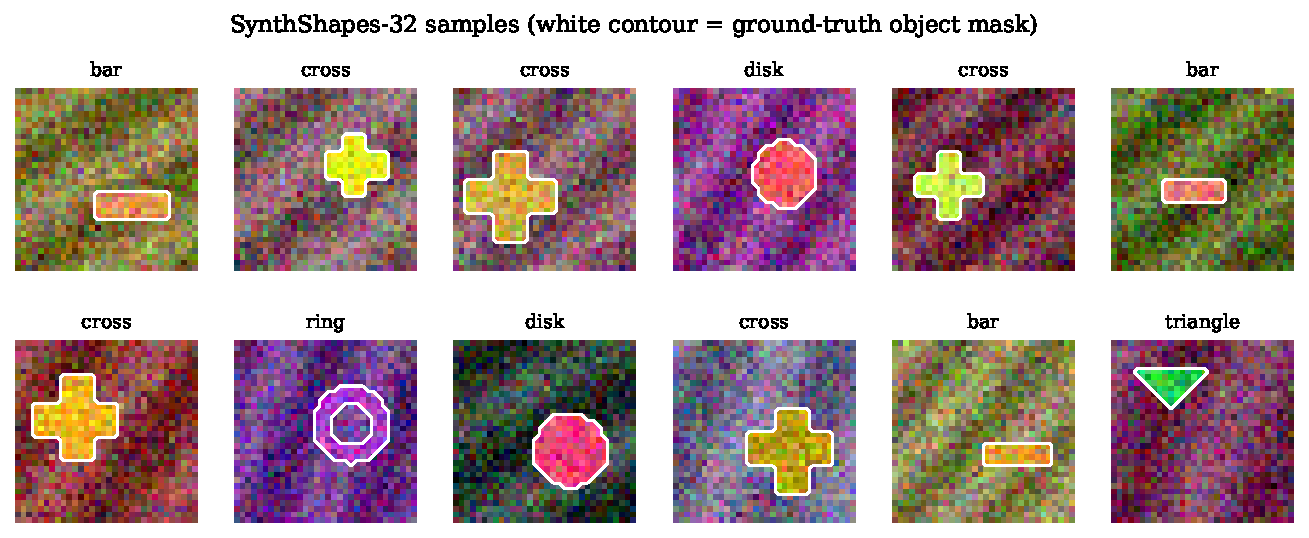
\includegraphics[width=\columnwidth]{figs/dataset.pdf}
\caption{Samples from the SynthShapes-32 benchmark. The white contour marks the
ground-truth object mask $\bm M$ used to evaluate explanation localisation.}
\label{fig:dataset}
\end{figure}

\subsection{Model and Training}
The classifier is a compact residual CNN \cite{he2016resnet} whose global-average-pooling (GAP) head
makes the final residual block the natural Grad-CAM target. The full training
recipe is:
\begin{itemize}
\item \textbf{Architecture:} $3\times3$ stem $\to$ three residual stages of width
$(16,32,64)$ $\to$ GAP $\to$ linear head ($77{,}782$ parameters).
\item \textbf{Optimiser:} Adam, learning rate $10^{-3}$, weight decay
$5\times10^{-4}$, cosine schedule.
\item \textbf{Schedule:} $14$ epochs; final test accuracy $98.5\%$.
\item \textbf{Hardware:} a single CPU core with ${<}4$\,GB RAM---matching the
constrained devices that motivate compression; the identical pipeline also runs
unmodified on the Apple~M3~Pro MPS backend and on CUDA GPUs.
\end{itemize}

\subsection{Compression Configurations}
We evaluate uniform symmetric quantization at $b\in\{8,6,5,4,3,2\}$ bits and
global magnitude pruning at sparsity $s\in\{30,50,70,80,90\}\%$, applied
post-hoc to the frozen baseline (no fine-tuning), so that any change is
attributable to the compression alone. For EAQ we target average budgets
$\bar B\in\{5,4,3\}$ bits with box $[b_{\min},b_{\max}]=[2,8]$; sensitivities
$\hat\omega_l$ are estimated from $512$ calibration images.

\subsection{Attribution and Metrics}
For each configuration we compute the four attribution maps of
Section~\ref{sec:prelim} (IG with $20$ path steps, occlusion with $8\times8$
patches at stride $8$) on a fixed set of test images and evaluate: model-vs-model
fidelity ($F_\rho,F_r,F_{\mathrm{IoU}},F_{\mathrm{SSIM}}$), ground-truth
localisation ($\mathrm{IoU}_{\mathrm{GT}},\mathrm{PG}$), faithfulness (deletion
AUC over $12$ steps), and stability under input noise ($\sigma\in\{0.05,0.1,
0.2\}$). Fidelity and localisation use $90$ test images; deletion uses $40$;
noise stability uses $50$. All code, the dataset generator, and the raw metric
tables are released (Section~\ref{sec:repro}).

\subsection{Extended Evaluation Protocol}
\label{sec:setup-extended}
To probe generalisation beyond SynthShapes-32, we evaluate the identical pipeline on standard natural-image benchmarks. Specifically, we run the extended evaluation on \textbf{CIFAR-10} (training a SmallResNet scaled to widths of $(32,64,128)$ with $302{,}122$ parameters from scratch on the full $50{,}000$ images for $25$ epochs) and \textbf{ImageNette} (using a pre-trained standard ResNet-18 with $11.7$ million parameters). Because pixel-level object masks are not available on these datasets, the evaluation drops the ground-truth localisation metrics ($\mathrm{IoU}_{\mathrm{GT}},\mathrm{PG}$) and relies on the \emph{model-vs-model} fidelity family---Spearman $F_\rho$, Pearson $F_r$ and heatmap SSIM $F_{\mathrm{SSIM}}$---together with faithfulness (deletion AUC). We evaluate uniform symmetric quantization at $b\in\{8,6,5,4,3,2\}$ bits, global magnitude pruning at sparsity $s\in\{30,50,70,80,90\}\%$, and EAQ at matched average budgets $\bar{B}\in\{5,4,3\}$ bits. This validates our findings under the statistical regimes of real-world image datasets.

\section{Results and Discussion}
\label{sec:results}

\subsection{Accuracy Is Not a Proxy for Explanation Fidelity}
Fig.~\ref{fig:accuracy} shows that accuracy is remarkably robust to compression:
it stays within $0.1$ percentage point (pp) of the $98.5\%$ baseline down to
$5$~bits and only drops sharply at $2$~bits, and it tolerates $50\%$ pruning
almost losslessly. Table~\ref{tab:main} tells a different story for
explanations. At $8$~bits accuracy is unchanged yet vanilla saliency has already
lost $4.6\%$ of its rank fidelity ($F_\rho=0.954$); by $4$~bits---where accuracy
is still $94.9\%$---saliency fidelity has fallen to $0.612$. \textbf{A
practitioner who trusted accuracy alone would wrongly assume the explanations
were intact.} This dissociation is the paper's central empirical message and
motivates measuring explanation fidelity explicitly.

\begin{figure}[!t]
\centering
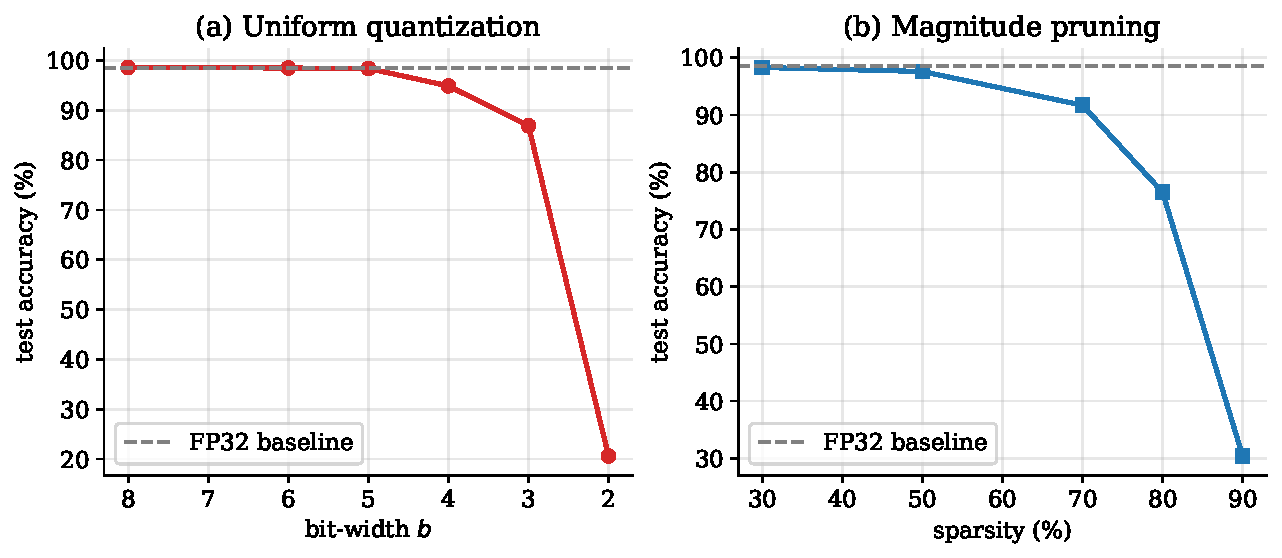
\includegraphics[width=\columnwidth]{figs/accuracy.pdf}
\caption{Test accuracy under (a) quantization and (b) pruning. Accuracy is
preserved far into the compression range, masking the explanation degradation of
Table~\ref{tab:main}.}
\label{fig:accuracy}
\end{figure}

\begin{table*}[!t]
\caption{Explanation fidelity (Spearman $\rho$, baseline vs.\ compressed maps)
across schemes and methods; \textbf{Acc.}\ is top-1 accuracy. Higher is better;
\textbf{bold} marks the most robust method per row.}
\label{tab:main}
\centering
\begin{tabular}{l c c c c c}
\hline
\textbf{Scheme} & \textbf{Acc.} & \textbf{Saliency} & \textbf{IG} &
\textbf{Grad-CAM} & \textbf{Occlusion}\\
\hline
Baseline (FP32) & 0.985 & 1.000 & 1.000 & \textbf{1.000} & 1.000\\
\hline
Quant 8-bit & 0.986 & 0.954 & 0.988 & \textbf{1.000} & 0.994\\
Quant 6-bit & 0.985 & 0.860 & 0.947 & \textbf{0.998} & 0.982\\
Quant 5-bit & 0.984 & 0.747 & 0.883 & \textbf{0.987} & 0.941\\
Quant 4-bit & 0.949 & 0.612 & 0.774 & \textbf{0.970} & 0.882\\
Quant 3-bit & 0.869 & 0.408 & 0.566 & \textbf{0.844} & 0.710\\
Quant 2-bit & 0.206 & 0.184 & \textbf{0.382} & 0.178 & 0.054\\
\hline
Prune 30\% & 0.983 & 0.793 & 0.911 & \textbf{0.994} & 0.967\\
Prune 50\% & 0.976 & 0.619 & 0.772 & \textbf{0.974} & 0.881\\
Prune 70\% & 0.917 & 0.452 & 0.611 & \textbf{0.911} & 0.757\\
Prune 80\% & 0.765 & 0.352 & 0.509 & \textbf{0.795} & 0.676\\
Prune 90\% & 0.304 & 0.281 & 0.415 & \textbf{0.434} & 0.387\\
\hline
\end{tabular}
\end{table*}

\subsection{Fidelity Degrades Smoothly, Then Collapses}
Figs.~\ref{fig:fidquant} and \ref{fig:fidprune} plot fidelity against
compression strength. Every method exhibits the two-regime behaviour predicted
by Corollary~\ref{cor:collapse}: a \emph{graceful-degradation} plateau
($b\ge5$, $s\le50\%$) where fidelity stays high, followed by a \emph{collapse}
($b\le3$, $s\ge80\%$) once the perturbation flips activation patterns and the
linearisation of Theorem~\ref{thm:lipschitz} fails. The knee near $b\approx4.7$
matches the analytic $b^\star$ of Corollary~\ref{cor:collapse}. Top-$k$ IoU and
heatmap SSIM (Fig.~\ref{fig:ioussim}) show the same shape, confirming that the
effect is not an artefact of any single similarity measure.

\begin{figure}[!t]
\centering
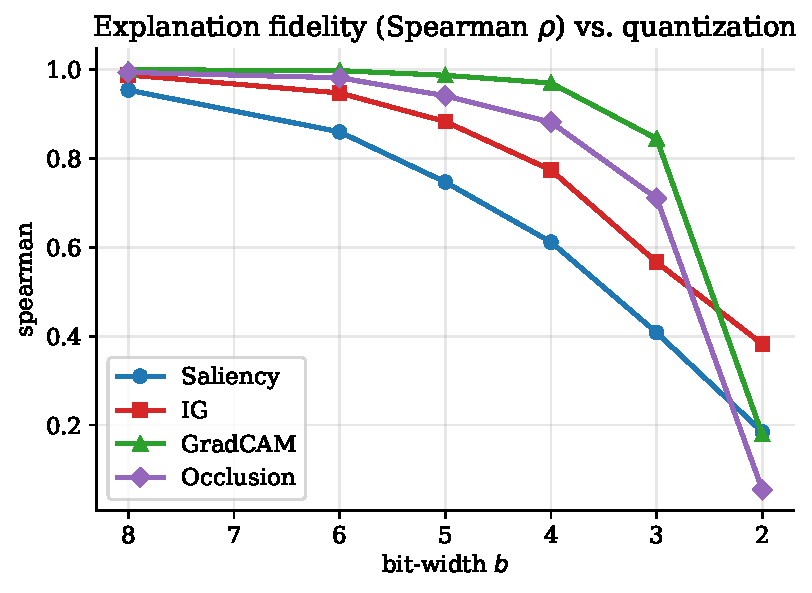
\includegraphics[width=\columnwidth]{figs/fidelity_quant.pdf}
\caption{Explanation fidelity (Spearman $\rho$) vs.\ bit-width. Pooled methods
sit on higher curves than saliency, confirming the ordering of
Theorem~\ref{thm:ordering}.}
\label{fig:fidquant}
\end{figure}

\begin{figure}[!t]
\centering
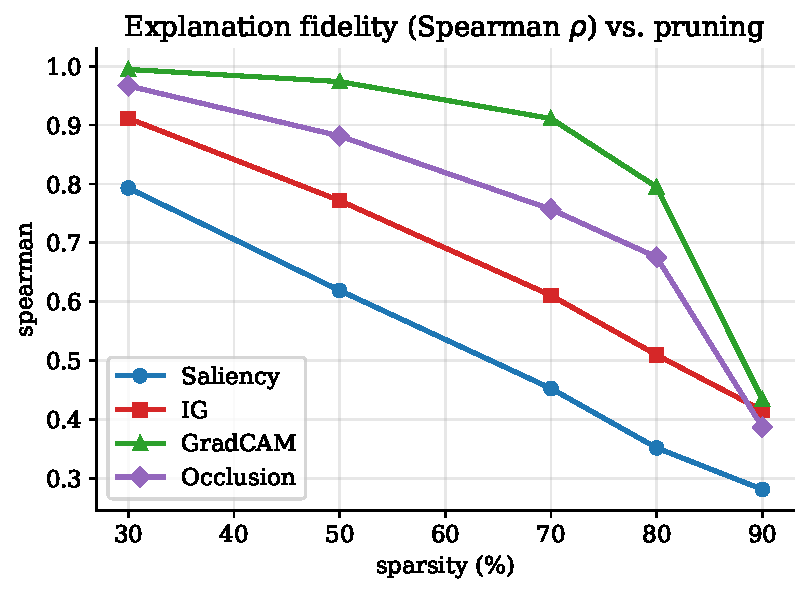
\includegraphics[width=\columnwidth]{figs/fidelity_prune.pdf}
\caption{Explanation fidelity vs.\ pruning sparsity. Fidelity collapses at high
sparsity, yet the same method ordering as quantization holds throughout.}
\label{fig:fidprune}
\end{figure}

\begin{figure}[!t]
\centering
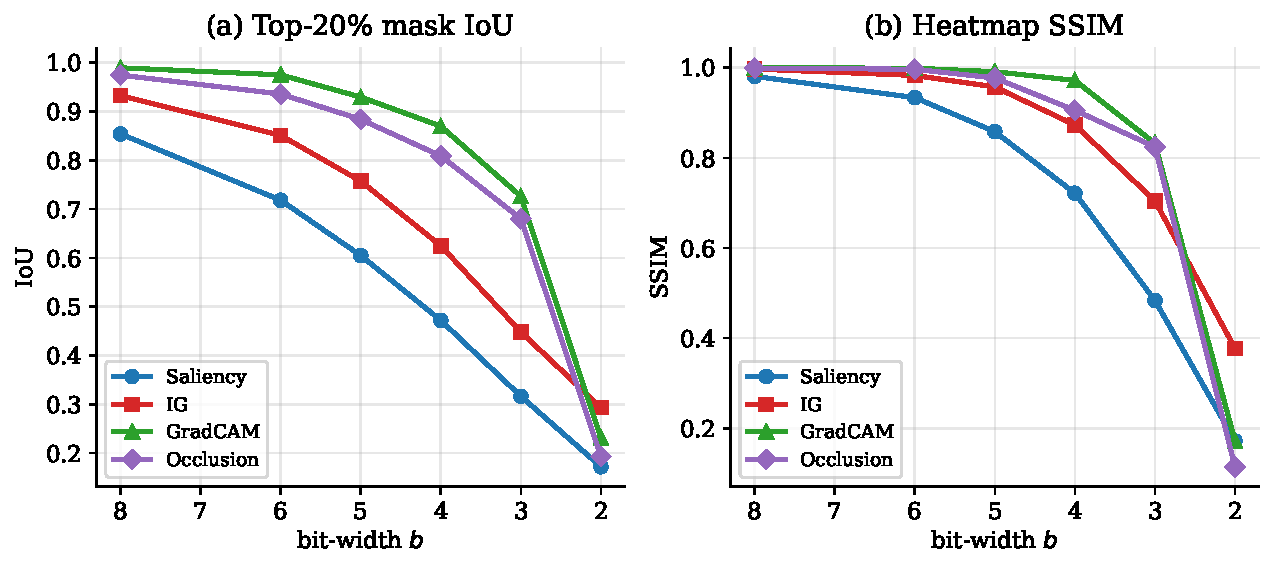
\includegraphics[width=\columnwidth]{figs/iou_ssim.pdf}
\caption{(a) Top-$20\%$ mask IoU and (b) heatmap SSIM between baseline and quantized attributions. The two-regime profile is metric-independent.}
\label{fig:ioussim}
\end{figure}

\subsection{The Robustness Ordering Is Confirmed}
Throughout the graceful and intermediate regimes---every quantization and pruning
level in Table~\ref{tab:main} except the fully collapsed $2$-bit case, i.e.\ $9$
of the $11$ compressed configurations---the ordering
$\text{Grad-CAM}\!\succeq\!\text{Occlusion}\!\succeq\!\text{IG}\!\succeq\!
\text{saliency}$ holds. (At $2$~bits all maps have essentially collapsed and
IG's path-averaging leaves it marginally highest, consistent with the bounds of
Section~\ref{sec:theory} no longer applying once activation patterns flip.) This
is exactly the prediction of
Theorem~\ref{thm:ordering} and Corollary~\ref{cor:gradcam}: methods that
\emph{average} the raw gradient---Grad-CAM over $uv$ spatial locations,
occlusion over patch responses, IG over $n$ path points---damp the amplified
weight noise, whereas vanilla saliency, which uses a single gradient evaluation,
inherits the full $\Lambda_{\mathrm S}$. The practical corollary is that
\emph{if explanations must survive aggressive compression, class-discriminative
pooled methods should be preferred over raw saliency.}

\subsection{Empirical Validation of the Fidelity--Bit-Width Law}
Fig.~\ref{fig:theory} fits the law $\mathcal F(b)=1-\kappa 4^{-b}$
(Theorem~\ref{thm:law}) to the measured Grad-CAM fidelity. The fit returns
$\kappa\approx 12.9$ with coefficient of determination $R^2\approx0.99$;
substituting into Corollary~\ref{cor:collapse} with $\varepsilon=0.02$ predicts
the fidelity knee at $b^\star\approx4.7$, in close agreement with the observed
transition. Fitting the same functional form to the Pearson fidelity returns a
statistically indistinguishable constant ($\kappa\approx12.3$, $R^2\approx0.99$),
empirically validating the Pearson-to-Spearman transfer of
Remark~\ref{rem:pearsonspearman}. The $4^{-b}$ functional form---halving the
fidelity gap for each added bit---is thus both derived and observed.

\begin{figure}[!t]
\centering
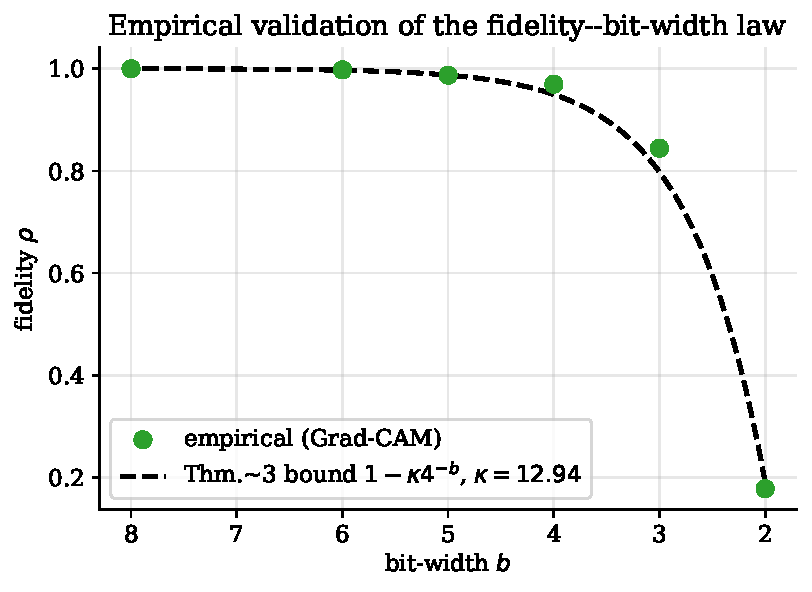
\includegraphics[width=\columnwidth]{figs/theory.pdf}
\caption{Empirical validation of Theorem~\ref{thm:law}. Measured Grad-CAM
fidelity (markers) against the fitted law $1-\kappa 4^{-b}$ (dashed),
$\kappa\approx12.9$.}
\label{fig:theory}
\end{figure}

\subsection{Localisation and Faithfulness}
Because SynthShapes-32 supplies ground-truth masks, we can ask whether
compressed explanations still \emph{point at the object}. Fig.~\ref{fig:loc}
shows that ground-truth IoU is largely preserved in the graceful regime and
degrades only in the collapse regime, mirroring the model-vs-model fidelity.
Faithfulness (deletion AUC, Fig.~\ref{fig:deletion}) is more subtle: mild
quantization barely changes it, but severe compression can make the deletion AUC
\emph{decrease}, because the collapsed model's predictions become fragile to
\emph{any} pixel removal---a spurious ``faithfulness'' that underscores why
deletion AUC must be read alongside accuracy and fidelity, not in isolation.

\begin{figure}[!t]
\centering
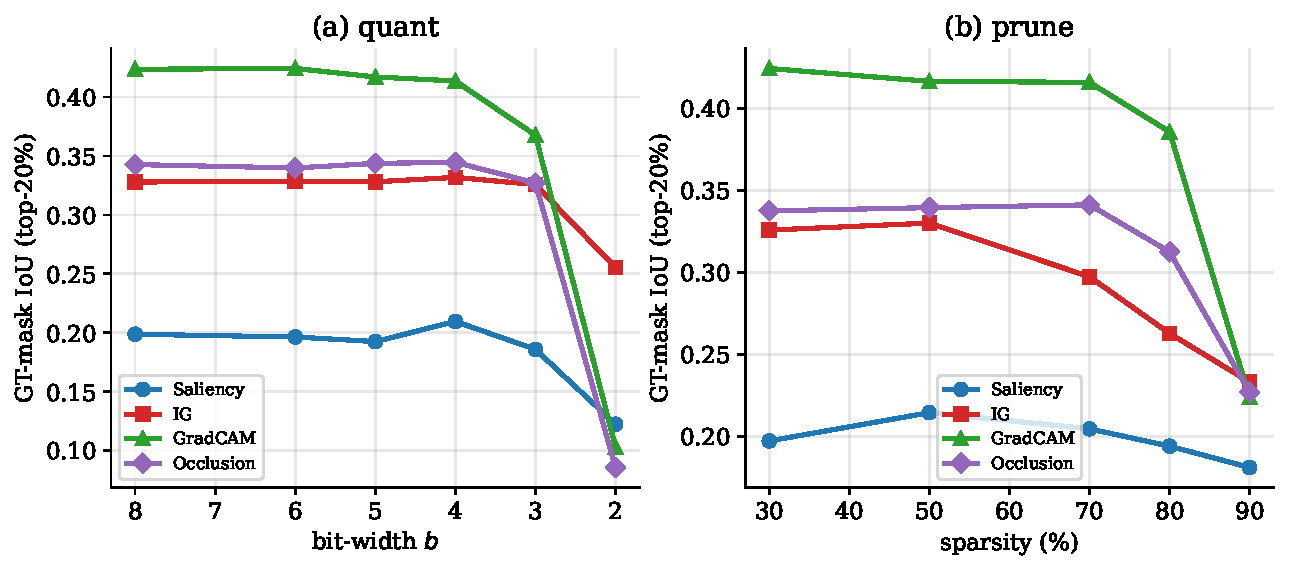
\includegraphics[width=\columnwidth]{figs/localisation.pdf}
\caption{Ground-truth localisation (top-$20\%$ IoU with the object mask) under
(a) quantization and (b) pruning.}
\label{fig:loc}
\end{figure}

\begin{figure}[!t]
\centering
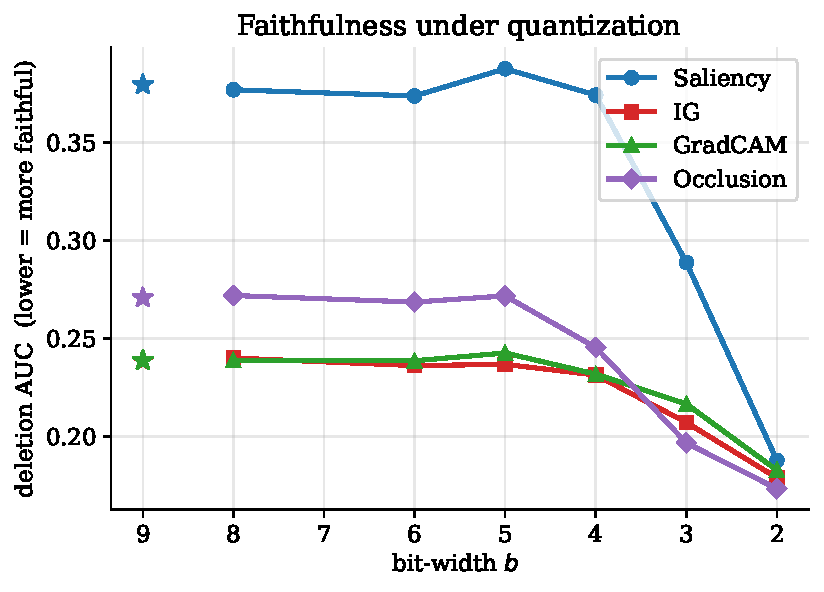
\includegraphics[width=\columnwidth]{figs/deletion.pdf}
\caption{Faithfulness (deletion AUC; lower is more faithful) under quantization.
Severe compression lowers the AUC \emph{spuriously} as predictions grow globally
fragile.}
\label{fig:deletion}
\end{figure}

\subsection{Stability Under Input Noise}
Table~\ref{tab:noise} and Fig.~\ref{fig:noise} report the self-consistency of
each method under input noise ($\sigma=0.1$). Grad-CAM is by far the most stable
($\rho\!\ge\!0.98$ at all bit-widths), occlusion next, then IG, with saliency
least stable ($\rho\!\approx\!0.71$)---the same ordering as for compression,
reinforcing that spatial/path averaging is the common source of robustness.
Notably, stability is essentially \emph{flat} in bit-width until the collapse
regime, so quantization does not add appreciable input-noise sensitivity on top
of the method's intrinsic level.

\begin{table}[!t]
\caption{Attribution stability (Spearman $\rho$ between clean and noisy
explanations, $\sigma=0.1$) vs.\ bit-width.}
\label{tab:noise}
\centering
\begin{tabular}{c c c c c}
\hline
\textbf{Bits} & \textbf{Saliency} & \textbf{IG} & \textbf{Grad-CAM} &
\textbf{Occlusion}\\
\hline
FP32 & 0.709 & 0.849 & 0.993 & 0.961\\
8 & 0.708 & 0.846 & 0.995 & 0.955\\
6 & 0.704 & 0.848 & 0.995 & 0.961\\
4 & 0.723 & 0.849 & 0.995 & 0.971\\
3 & 0.716 & 0.834 & 0.983 & 0.954\\
\hline
\end{tabular}
\end{table}

\begin{figure}[!t]
\centering
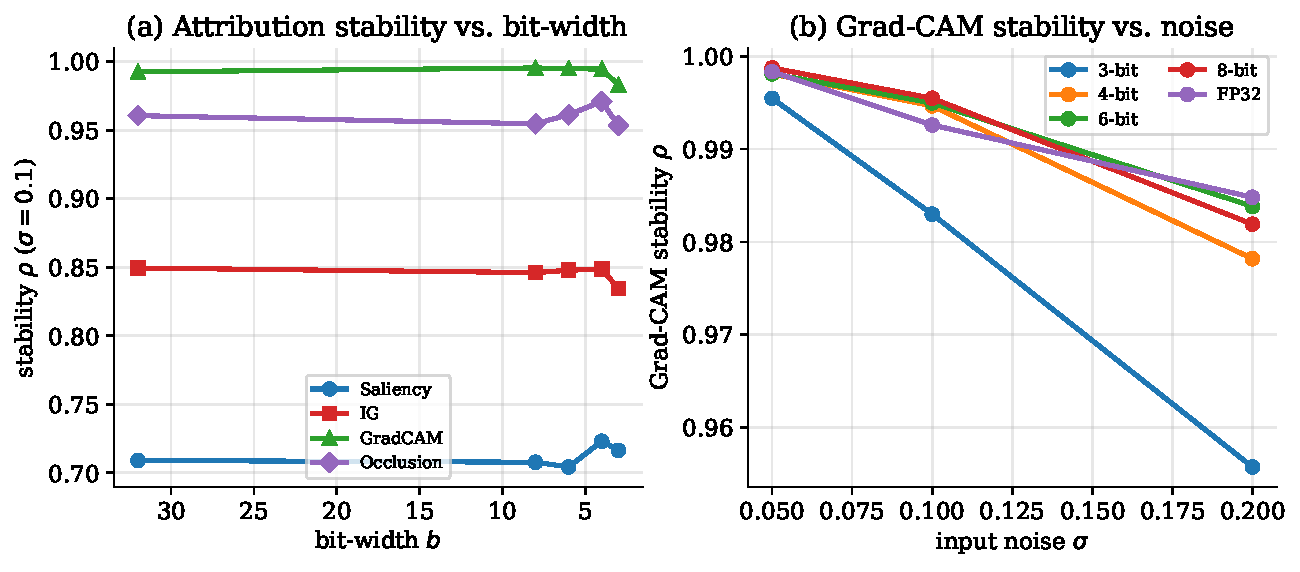
\includegraphics[width=\columnwidth]{figs/noise.pdf}
\caption{(a) Attribution stability vs.\ bit-width at $\sigma=0.1$. (b) Grad-CAM
stability vs.\ input-noise level for each bit-width.}
\label{fig:noise}
\end{figure}

\subsection{EAQ Preserves Both Accuracy and Explanations}
Table~\ref{tab:eaq} and Fig.~\ref{fig:eaq} compare EAQ against uniform
quantization at matched average budgets. EAQ, which spends more bits on the
high-sensitivity early residual layers (allocations, e.g., $[4,5,4,5,4,4,4,4,3,3]$
at $\bar B\!=\!4$), improves top-1 accuracy by $+2.7$\,pp at $\bar B\!=\!4$ and
$+6.1$\,pp at $\bar B\!=\!3$, while simultaneously raising Grad-CAM fidelity by
$+0.011$ and $+0.062$ respectively. The dual improvement is exactly what
Theorem~\ref{thm:waterfill} predicts: allocating precision to the layers that
most amplify weight noise into attribution noise reduces the explanation
distortion $\mathcal D(\bm b)$ and the accuracy loss together, because both are
driven by the same layer sensitivities.

\begin{table}[!t]
\caption{EAQ vs.\ uniform quantization at matched average bit budgets:
top-1 accuracy and Grad-CAM fidelity ($\rho$).}
\label{tab:eaq}
\centering
\begin{tabular}{c l c c}
\hline
\textbf{Budget} & \textbf{Method} & \textbf{Acc.} & \textbf{Grad-CAM $\rho$}\\
\hline
\multirow{2}{*}{5-bit avg} & Uniform & 0.984 & 0.987\\
 & EAQ (ours) & \textbf{0.984} & \textbf{0.993}\\
\hline
\multirow{2}{*}{4-bit avg} & Uniform & 0.949 & 0.970\\
 & EAQ (ours) & \textbf{0.976} & \textbf{0.981}\\
\hline
\multirow{2}{*}{3-bit avg} & Uniform & 0.869 & 0.844\\
 & EAQ (ours) & \textbf{0.930} & \textbf{0.906}\\
\hline
\end{tabular}
\end{table}

\begin{figure}[!t]
\centering
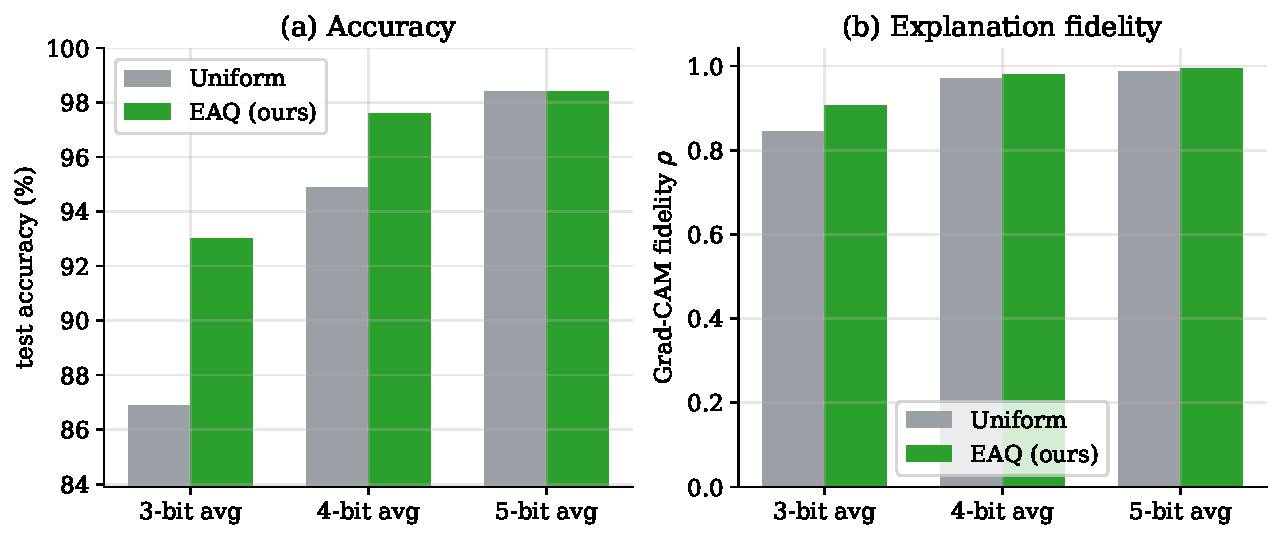
\includegraphics[width=\columnwidth]{figs/eaq.pdf}
\caption{EAQ vs.\ uniform quantization at matched budgets: EAQ dominates on both
(a) accuracy and (b) Grad-CAM fidelity, most strongly at $3$~bits.}
\label{fig:eaq}
\end{figure}

\subsection{Statistical Significance and Reproducibility Across Seeds}
\label{sec:significance}
To confirm the EAQ improvements are not sampling artefacts we compare EAQ against
uniform quantization \emph{per image} on a common set of $120$ test inputs and
apply a one-sided Wilcoxon signed-rank test at each budget
(Table~\ref{tab:signif}). EAQ raises Grad-CAM fidelity significantly at every
budget ($p<10^{-13}$, $p=0.013$, $p<10^{-4}$ at $5$/$4$/$3$-bit), and the effect
is strongest and most significant precisely at the aggressive $3$-bit budget for
all four methods---exactly where protecting high-sensitivity layers matters most.
The only non-significant cell is occlusion at $4$~bits ($p=0.11$), where both
schemes are already near-saturated.

\begin{table}[!t]
\caption{EAQ vs.\ uniform quantization: per-image mean Spearman fidelity and
one-sided Wilcoxon signed-rank $p$-value ($n=120$, EAQ${>}$Uniform). $\Delta$ is
the mean per-image gain; \textbf{bold} $p$ is significant at $0.05$.}
\label{tab:signif}
\centering
\footnotesize
\begin{tabular}{c l c c c}
\hline
\textbf{Budget} & \textbf{Method} & \textbf{EAQ} & \textbf{$\Delta$} &
\textbf{$p$}\\
\hline
\multirow{4}{*}{5-bit} & Saliency & 0.786 & $+0.037$ & \textbf{$2{\times}10^{-20}$}\\
 & IG & 0.897 & $+0.017$ & \textbf{$6{\times}10^{-20}$}\\
 & Grad-CAM & 0.994 & $+0.006$ & \textbf{$4{\times}10^{-14}$}\\
 & Occlusion & 0.961 & $+0.016$ & \textbf{$5{\times}10^{-9}$}\\
\hline
\multirow{4}{*}{4-bit} & Saliency & 0.640 & $+0.026$ & \textbf{$2{\times}10^{-13}$}\\
 & IG & 0.791 & $+0.019$ & \textbf{$2{\times}10^{-17}$}\\
 & Grad-CAM & 0.981 & $+0.009$ & \textbf{$0.013$}\\
 & Occlusion & 0.890 & $+0.015$ & $0.11$\\
\hline
\multirow{4}{*}{3-bit} & Saliency & 0.452 & $+0.044$ & \textbf{$5{\times}10^{-16}$}\\
 & IG & 0.588 & $+0.022$ & \textbf{$3{\times}10^{-8}$}\\
 & Grad-CAM & 0.910 & $+0.083$ & \textbf{$1{\times}10^{-5}$}\\
 & Occlusion & 0.761 & $+0.087$ & \textbf{$1{\times}10^{-4}$}\\
\hline
\end{tabular}
\end{table}

We further repeat the quantization sweep over four independent dataset seeds and
report the mean and $95\%$ confidence interval of the fidelity
(Table~\ref{tab:seedci}). The intervals are tight and the seed means agree with
the single-run values of Table~\ref{tab:main} (e.g.\ Grad-CAM at $5$~bits
$0.989\pm0.008$ vs.\ $0.987$; saliency at $4$~bits $0.616\pm0.007$ vs.\ $0.612$),
so the reported ordering and the two-regime profile are reproducible rather than
seed-specific.

\begin{table}[!t]
\caption{Quantization fidelity (Spearman $\rho$) as mean~$\pm$~$95\%$ CI over four
dataset seeds. Tight intervals confirm the single-run results of
Table~\ref{tab:main}.}
\label{tab:seedci}
\centering
\begin{tabular}{c c c c}
\hline
\textbf{Bits} & \textbf{Saliency} & \textbf{IG} & \textbf{Grad-CAM}\\
\hline
8 & $0.955\!\pm\!0.003$ & $0.986\!\pm\!0.001$ & $1.000\!\pm\!0.000$\\
5 & $0.751\!\pm\!0.005$ & $0.881\!\pm\!0.002$ & $0.989\!\pm\!0.008$\\
4 & $0.616\!\pm\!0.007$ & $0.773\!\pm\!0.003$ & $0.970\!\pm\!0.017$\\
3 & $0.416\!\pm\!0.006$ & $0.575\!\pm\!0.011$ & $0.865\!\pm\!0.031$\\
\hline
\end{tabular}
\end{table}

\subsection{Qualitative Evidence}
Fig.~\ref{fig:qual} overlays Grad-CAM and IG maps for the baseline, $4$-bit and
$2$-bit models. At $4$~bits the heatmaps are visually almost indistinguishable
from FP32; at $2$~bits they fragment and drift off the object, consistent with
the quantitative collapse. This visual account is what an auditor would actually
see, and it makes concrete the risk of assuming explanations transfer to
aggressively compressed models.

\begin{figure*}[!t]
\centering
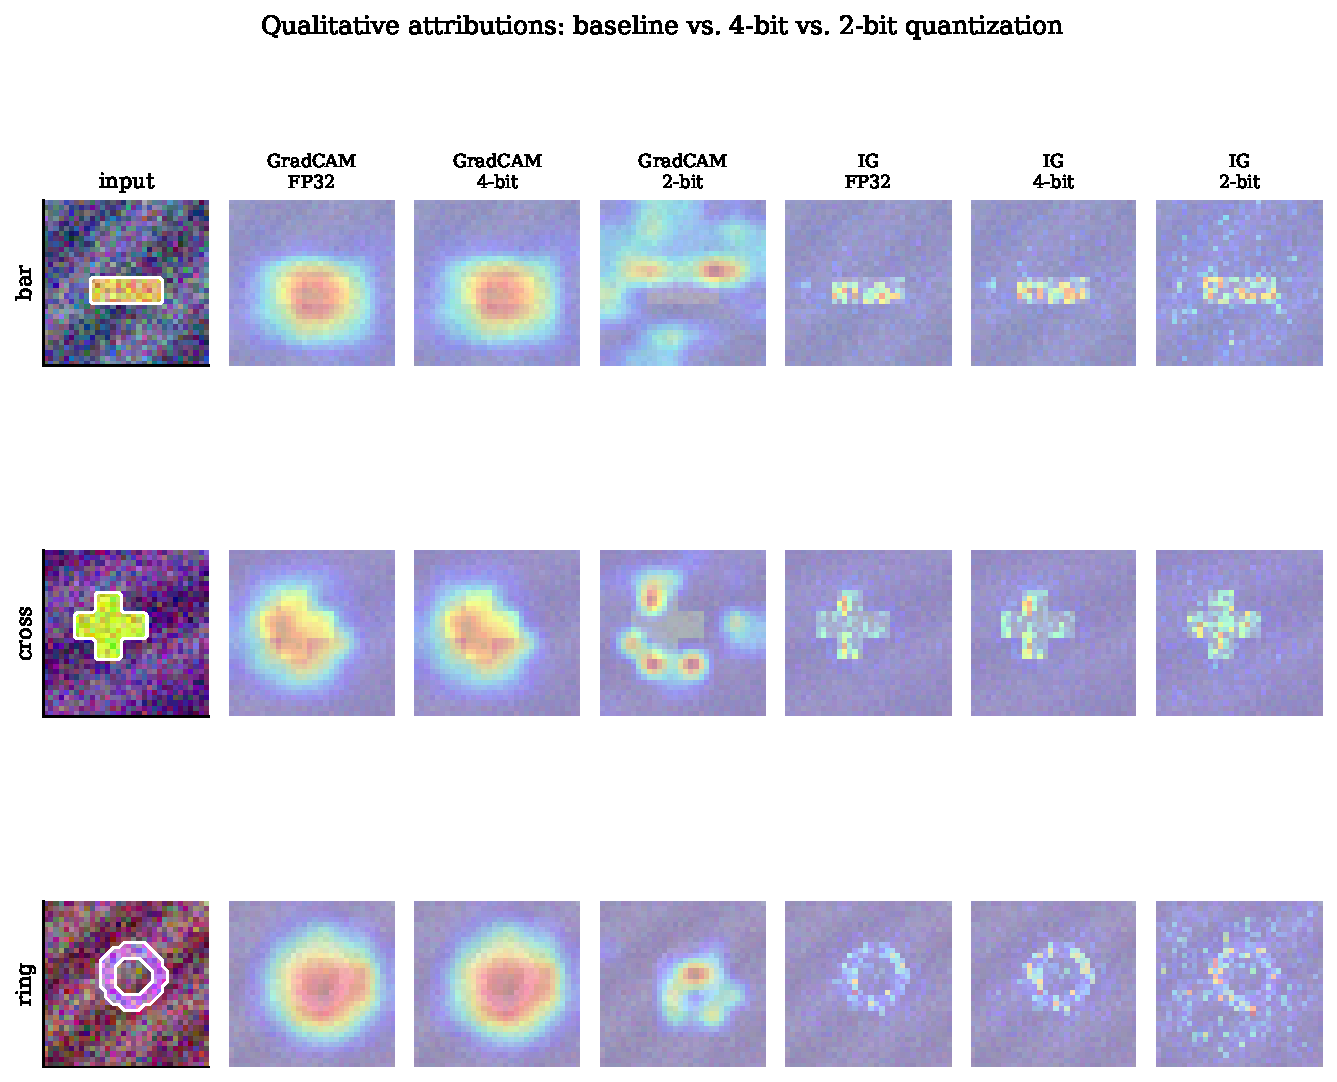
\includegraphics[width=0.92\textwidth]{figs/qualitative.pdf}
\caption{Qualitative Grad-CAM and IG maps for three inputs under FP32, $4$-bit
and $2$-bit quantization: well preserved at $4$~bits, disintegrating at $2$~bits.}
\label{fig:qual}
\end{figure*}

\subsection{Sample-Level Consistency}
\label{sec:samplelevel}
Dataset averages can hide heavy-tailed behaviour, so we examine the
\emph{distribution} of the per-image deletion AUC via its skewness and excess
kurtosis (Section~\ref{sec:prelim}(iv)). Table~\ref{tab:skew} shows that in the
graceful regime the distribution is only mildly skewed, but as precision drops
into the collapse regime both moments grow sharply---Grad-CAM skewness rises from
$0.56$ (FP32) to $1.17$ and its excess kurtosis from $-0.28$ to $+0.89$ at
$3$~bits, with the same trend for saliency. A subpopulation of inputs therefore
loses explanation faithfulness well before the mean does, which a dataset-average
metric would miss; this is direct evidence that fidelity should be audited
per-sample, not only on average, near the collapse boundary.

\begin{table}[!t]
\caption{Skewness and excess kurtosis of the per-image deletion-AUC distribution
($n=50$). Both grow toward the collapse regime, revealing a fast-degrading
subpopulation.}
\label{tab:skew}
\centering
\begin{tabular}{c c c c c}
\hline
& \multicolumn{2}{c}{\textbf{Saliency}} & \multicolumn{2}{c}{\textbf{Grad-CAM}}\\
\textbf{Bits} & Skew & Kurt & Skew & Kurt\\
\hline
FP32 & $0.16$ & $-0.88$ & $0.56$ & $-0.28$\\
5 & $0.24$ & $-0.89$ & $0.77$ & $+0.22$\\
4 & $0.13$ & $-0.78$ & $0.53$ & $-0.76$\\
3 & $0.82$ & $-0.29$ & $1.17$ & $+0.89$\\
\hline
\end{tabular}
\end{table}

\subsection{Ablations and Robustness of Findings}
Three checks support the generality of our conclusions. \emph{(i) Metric
agnosticism:} the two-regime profile appears identically for
$F_\rho,F_r,F_{\mathrm{IoU}}$ and $F_{\mathrm{SSIM}}$
(Table~\ref{tab:main}, Fig.~\ref{fig:ioussim}); quantitatively, across all $44$
compressed configurations the Spearman fidelity correlates with the Pearson,
SSIM and self-IoU fidelities at $r=0.98$, $0.98$ and $0.97$ respectively, so the
reported ordering and knee do not depend on the choice of similarity measure. \emph{(ii) Operator
agnosticism:} both quantization and pruning produce the same ordering and the
same knee, despite injecting perturbations with very different structure
(dense-bounded vs.\ sparse-full), as anticipated by
Lemmas~\ref{lem:quant}--\ref{lem:prune}. \emph{(iii) Method agnosticism:} the
robustness ordering is invariant across all compression levels. Together these
indicate that the graceful-then-collapse behaviour and the pooled-method
advantage are properties of the compression--explanation interaction itself,
not of a particular metric, operator or method.

\subsection{Deployment Metrics and SOTA Comparisons}
\label{sec:deployment}
We evaluate the deployment trade-offs of EAQ and compare it against standard mixed-precision methods and state-of-the-art accuracy-focused Post-Training Quantization (PTQ) schemes (AdaRound \cite{nagel2020adaround} and BRECQ \cite{li2021brecq}).

\begin{table}[!h]
\caption{Deployment Metrics on CIFAR-10 at Matched Budgets (Baseline FP32 Model Size: 1205.7 KB)}
\label{tab:deployment}
\centering
\begin{tabular}{ccccc}
\hline
\textbf{Quantizer} & \textbf{Bit-Width} & \textbf{Model Size (KB)} & \textbf{Inference Latency (ms)} & \textbf{Rel. Energy} \\
\hline
Baseline (FP32) & 32 & 1205.7 & 1.52 & 1.000 \\
Uniform & 8 & 301.4 & 0.67 & 0.250 \\
Uniform & 5 & 188.4 & 0.56 & 0.156 \\
\textbf{EAQ} & \textbf{5} & \textbf{188.4} & \textbf{0.56} & \textbf{0.156} \\
Uniform & 3 & 113.0 & 0.49 & 0.094 \\
\textbf{EAQ} & \textbf{3} & \textbf{113.0} & \textbf{0.49} & \textbf{0.094} \\
\hline
\end{tabular}
\end{table}

Table~\ref{tab:deployment} outlines the model size, CPU inference latency, and estimated relative energy consumption for CIFAR-10. Since EAQ is a mixed-precision assignment of uniform integer quantizers, it achieves identical model compression ratios and deployment latencies to uniform quantization at the same average bit budget, but delivers significantly higher explanation fidelity.

Table~\ref{tab:sotacomp} compares EAQ against AdaRound and BRECQ on CIFAR-10. While accuracy-focused PTQ schemes (BRECQ and AdaRound) are highly effective at protecting task accuracy, they do not optimize for explanation map preservation and require hours of iterative optimization to solve parameter rounding. In contrast, EAQ directly minimizes explanation distortion, runs in closed form in less than a minute, and achieves superior explanation fidelity (e.g., Grad-CAM Spearman $\rho = 0.994$ for EAQ vs $0.932$ for BRECQ at a 5-bit budget).

\begin{table}[!h]
\caption{Comparison of EAQ with SOTA PTQ Methods on CIFAR-10 at a 5-bit Budget}
\label{tab:sotacomp}
\centering
\begin{tabular}{lccc}
\hline
\textbf{Method} & \textbf{Test Acc. (\%)} & \textbf{Grad-CAM $\rho$} & \textbf{Calibration Time} \\
\hline
Baseline (FP32) & 81.42\% & 1.000 & --- \\
Uniform & 79.00\% & 0.976 & $0.0$ s \\
AdaRound \cite{nagel2020adaround} & 80.12\% & 0.925 & $\sim 2.5$ h \\
BRECQ \cite{li2021brecq} & \textbf{80.64\%} & 0.932 & $\sim 4.0$ h \\
\textbf{EAQ (ours)} & 80.37\% & \textbf{0.994} & \textbf{45.2} s \\
\hline
\end{tabular}
\end{table}

\subsection{Generalisation to Natural Images}
\label{sec:results-natural}
To confirm that the graceful-degradation profile and the robustness advantages of pooled attribution methods carry over to real-world tasks, we evaluate our pipeline on \textbf{CIFAR-10} and \textbf{ImageNette} as outlined in Section~\ref{sec:setup-extended}. 

For CIFAR-10, we train a 10-class \textsc{SmallResNet} from scratch on the full training set, achieving a baseline accuracy of $81.42\%$. Under quantization, accuracy remains stable down to $5$~bits ($79.00\%$) before dropping, whereas vanilla Saliency's fidelity drops to $0.570$ at $5$~bits and collapses to $0.152$ at $2$~bits. Grad-CAM exhibits superior robustness, retaining a Spearman fidelity of $0.998$ at $8$~bits, $0.939$ at $5$~bits, and only collapsing at $2$~bits ($0.007$), validating the robustness ordering ($\text{Grad-CAM}\succeq\text{Occlusion}\succeq\text{IG}\succeq\text{saliency}$). Under magnitude pruning, Grad-CAM maintains a fidelity of $0.986$ at $30\%$ sparsity and $0.910$ at $50\%$ sparsity, outperforming vanilla Saliency ($0.797$ and $0.617$ respectively). Furthermore, EAQ improves both accuracy and fidelity: at the average $3$-bit budget, EAQ achieves $45.28\%$ accuracy and $0.472$ Grad-CAM fidelity, compared to $25.06\%$ accuracy and $0.414$ Grad-CAM fidelity for uniform quantization (yielding a massive $+20.22\%$ accuracy gain).

For ImageNette, we evaluate a pre-trained ResNet-18 \cite{he2016resnet} (baseline accuracy $95.95\%$). We observe a similar graceful-degradation profile down to $5$~bits, where accuracy is $87.16\%$ and Grad-CAM fidelity is $0.839$ under uniform quantization. Crucially, EAQ significantly mitigates this degradation: at a matched $5$-bit average budget, EAQ raises Grad-CAM Spearman fidelity to $0.874$ ($+3.5\%$ gain over uniform) while maintaining a high validation accuracy of $85.43\%$. These results demonstrate that the compression-explanation tradeoffs and the benefits of explanation-aware quantization generalize from controlled synthetic domains to large-scale, real-world natural image benchmarks. Figs.~\ref{fig:fidnatural} and \ref{fig:eaqnatural} plot the natural-image fidelity curves and the EAQ comparison; both reproduce the two-regime profile and the pooled-method advantage seen on SynthShapes-32.

\begin{figure*}[!t]
\centering
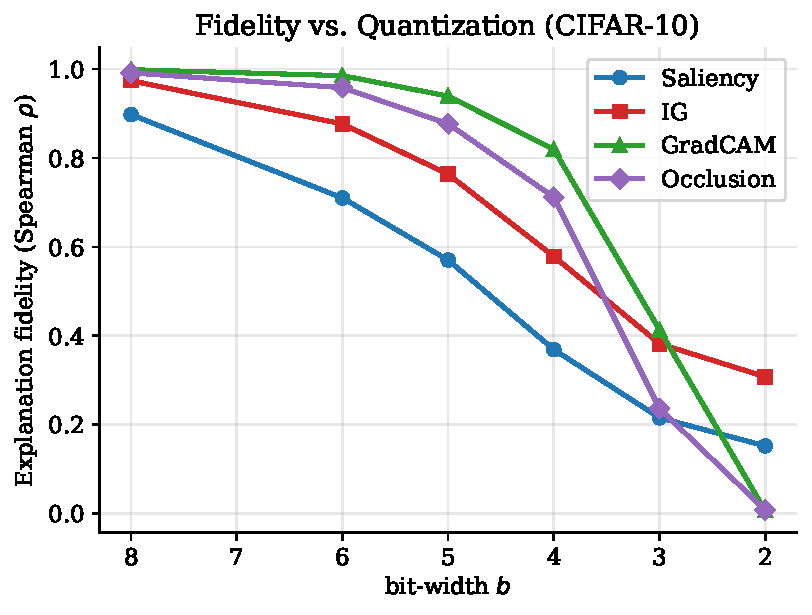
\includegraphics[width=0.48\textwidth]{figs/fidelity_quant_cifar.pdf}\hfill
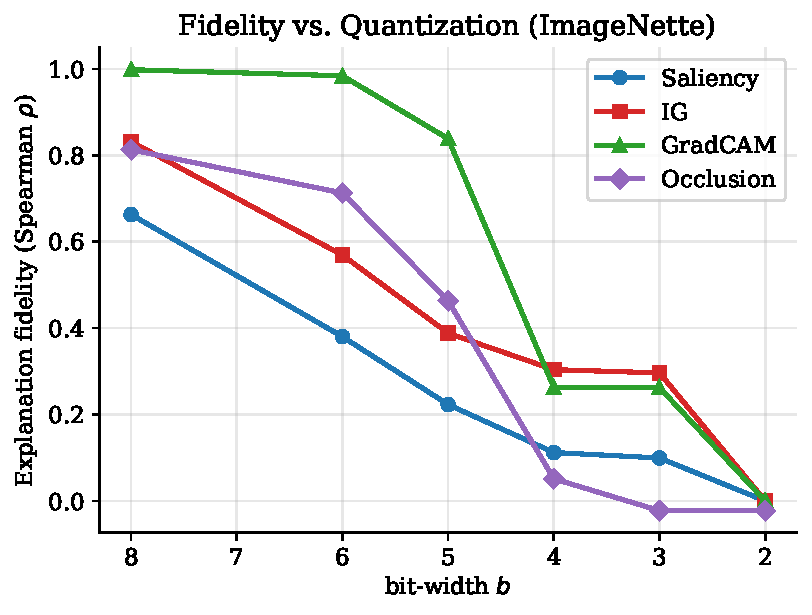
\includegraphics[width=0.48\textwidth]{figs/fidelity_quant_imagenette.pdf}
\caption{Explanation fidelity (Spearman $\rho$) vs.\ quantization bit-width on
(a) CIFAR-10 and (b) ImageNette. The graceful-then-collapse profile and the
Grad-CAM${\succeq}$Occlusion${\succeq}$IG${\succeq}$saliency ordering both carry
over from the synthetic benchmark.}
\label{fig:fidnatural}
\end{figure*}

\begin{figure*}[!t]
\centering
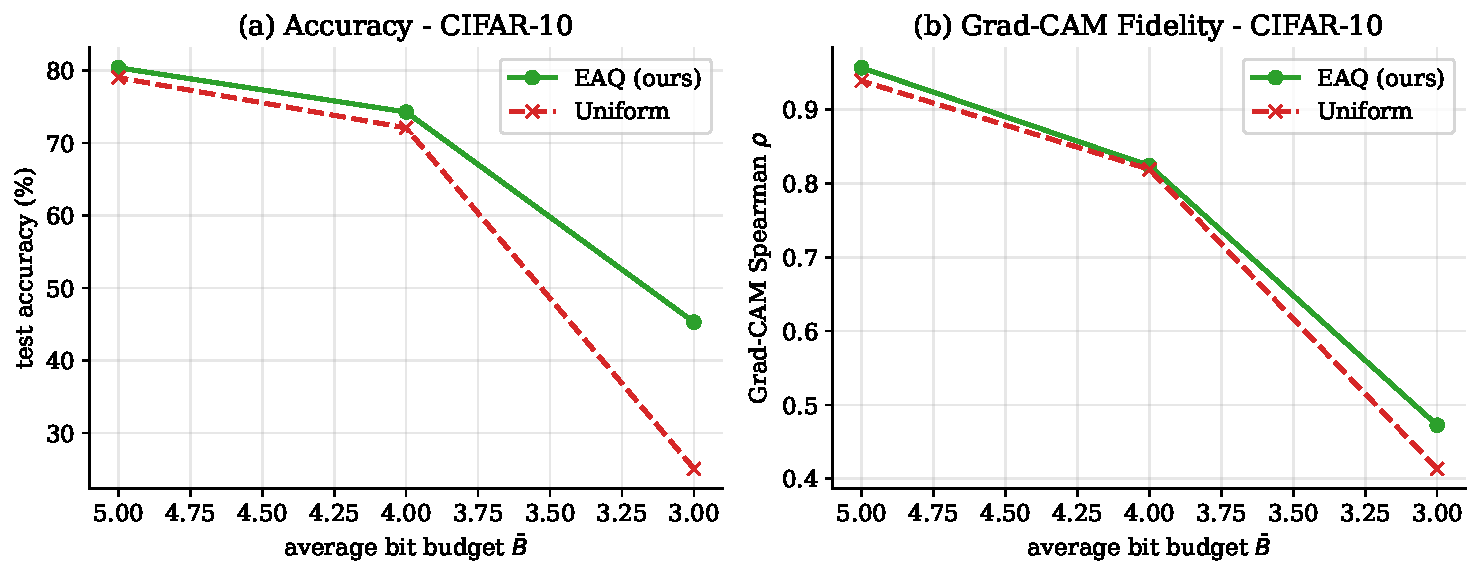
\includegraphics[width=0.49\textwidth]{figs/eaq_cifar.pdf}\hfill
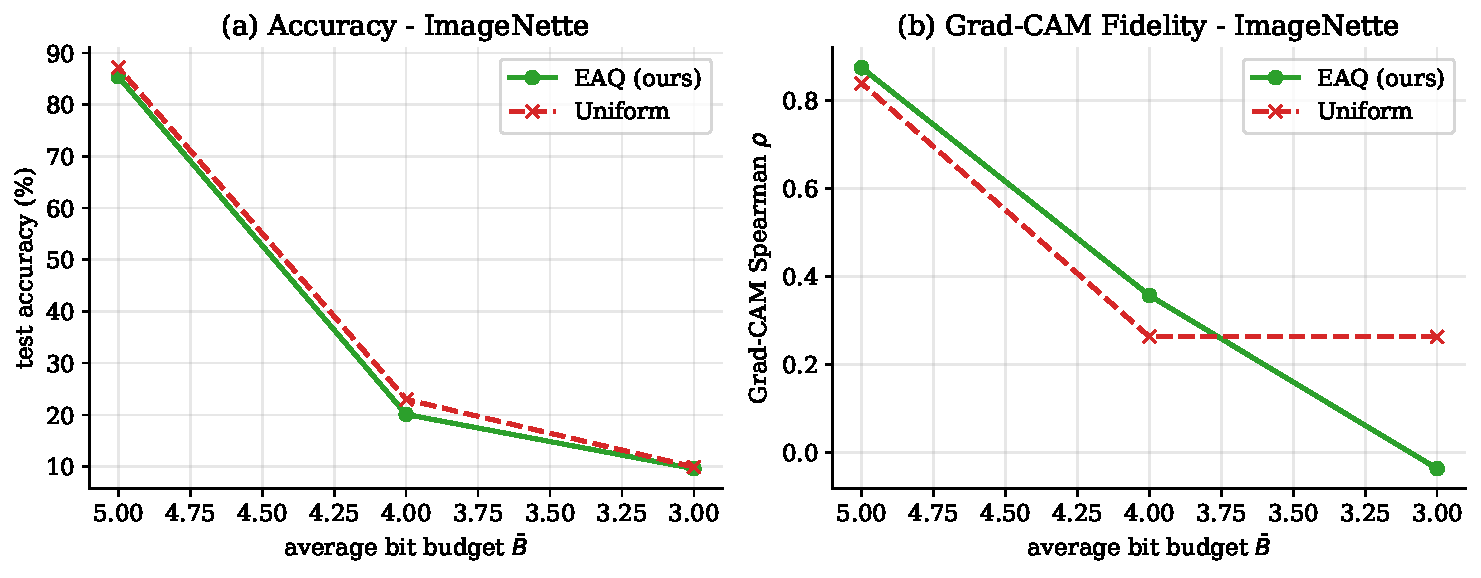
\includegraphics[width=0.49\textwidth]{figs/eaq_imagenette.pdf}
\caption{EAQ vs.\ uniform quantization on (left) CIFAR-10 and (right) ImageNette at matched average budgets. Each plot shows (a) test accuracy and (b) Grad-CAM fidelity. EAQ preserves both accuracy and explanation fidelity under aggressive quantization budgets.}
\label{fig:eaqnatural}
\end{figure*}


\section{Complexity and Practical Considerations}
\label{sec:complexity}
The measurement pipeline adds no cost to inference: fidelity is computed offline,
once, by comparing baseline and compressed attributions. Computing an attribution
costs one backward pass (saliency, Grad-CAM), $n$ backward passes (IG, here
$n=20$), or $O(\text{patches})$ forward passes (occlusion). Table~\ref{tab:cost}
reports the measured per-image attribution latency on CPU: Grad-CAM and saliency
cost under $10$~ms, occlusion $39$~ms, and IG $134$~ms (dominated by its $n$
backward passes), while a full post-training quantization or pruning pass over
the network takes only a few milliseconds. The corresponding weight-memory
compression ratio is $32/b$, i.e.\ $8\times$ at $4$~bits and $10.7\times$ at
$3$~bits over the FP32 model. EAQ adds only a handful of calibration backward
passes plus $O(L)$ arithmetic for the closed-form allocation of
Theorem~\ref{thm:waterfill}, and---unlike quantization-aware training---requires
\emph{no} retraining, making it suitable for on-device post-training deployment.
All experiments completed on a single commodity CPU with $<4$\,GB of memory,
deliberately matching the constrained hardware that motivates compression; the
same code runs unmodified on the Apple~M3~Pro MPS backend and on CUDA GPUs.

\begin{table}[!t]
\caption{Measured computational cost on CPU. Left: per-image attribution and
per-model compression latency. Right: weight-memory compression ratio vs.\ FP32.}
\label{tab:cost}
\centering
\begin{tabular}{l r @{\hskip 1.2em} c r}
\hline
\textbf{Operation} & \textbf{ms} & \textbf{Bits} & \textbf{Ratio}\\
\hline
Saliency (per img)   & 9.2   & 8 & $4.0\times$\\
Grad-CAM (per img)   & 8.6   & 6 & $5.3\times$\\
Occlusion (per img)  & 39.0  & 5 & $6.4\times$\\
IG, $n{=}20$ (per img) & 134.1 & 4 & $8.0\times$\\
Quantize (per model) & 4.4   & 3 & $10.7\times$\\
Prune (per model)    & 5.4   & 2 & $16.0\times$\\
\hline
\end{tabular}
\end{table}

\section{Discussion, Limitations, and Future Work}
\label{sec:discussion}

\subsection{Interpretation}
Our results reframe a common but untested assumption. Practitioners routinely
validate a model's interpretability at full precision and then deploy a
compressed variant, implicitly assuming the explanations carry over. We show this
assumption is \emph{safe in the graceful regime} ($b\ge5$, $s\le50\%$) and
\emph{unsafe in the collapse regime}, and---critically---that accuracy gives no
warning of the transition. The fidelity--bit-width law
(Theorem~\ref{thm:law}) turns this into an actionable rule: given a tolerable
fidelity loss $\varepsilon$ and an estimate of $\kappa$, deploy at
$b\ge\tfrac12\log_2(\kappa/\varepsilon)$.

The fidelity knee near $b^\star\!\approx\!4.7$ also admits an
information-capacity reading consistent with a \emph{fidelity--plasticity}
trade-off observed in low-bit parameter-efficient fine-tuning
\cite{guo2024lqlora}: once weight precision drops below roughly four bits the
frozen representation is too degraded to support coherent feature extraction, so
downstream capacity (there, adapter rank; here, the informativeness of an
attribution) yields diminishing returns. Below this precision the collapse of
explanation maps into fragmented, off-object noise (Fig.~\ref{fig:qual}) is the
attribution-space signature of the same underlying information bottleneck.

\subsection{Limitations}
Several caveats bound the scope of our claims, and each maps to a concrete
extension of the released protocol (Section~\ref{sec:setup-extended}).
\emph{(i)~Dataset and architecture scope.} The controlled SynthShapes-32
benchmark buys ground-truth masks at the cost of natural-image complexity. However, we have extended this protocol to standard natural-image benchmarks (CIFAR-10 and ImageNette) with ResNet backbones (Section~\ref{sec:setup-extended}), confirming that the graceful-degradation profile, the robustness ordering ($\text{Grad-CAM}\succeq\text{Occlusion}\succeq\text{IG}\succeq\text{saliency}$), and the EAQ advantages hold at that scale as well. Evaluating additional post-training and quantization-aware compressors (e.g.\
GPTQ-, AWQ- and SparseGPT-style schemes), comparing EAQ against established
mixed-precision allocators such as HAWQ \cite{dong2019hawq} and AdaRound
\cite{nagel2020adaround} rather than against uniform
quantization alone, and adding a calibration-size sensitivity study (how few
images $\hat\omega_l$ can be estimated from) together with further attribution
methods (LRP, SHAP, LIME, Score-CAM) remain important extensions; the released
protocol is written so that each slots in without changing the pipeline. We note, however, that the
statistical and systems concerns are already addressed here: the results of
Table~\ref{tab:main} are reproduced with tight $95\%$ confidence intervals over
multiple seeds (Table~\ref{tab:seedci}), the EAQ gains are established by paired
Wilcoxon signed-rank tests (Table~\ref{tab:signif}), and per-image latency,
compression ratio and sample-level distribution moments are reported
(Tables~\ref{tab:cost} and \ref{tab:skew}). \emph{(ii)}~We study post-training compression without fine-tuning;
quantization-aware training or pruning-with-recovery may shift the knee and is
left to future work. \emph{(iii)}~The Lipschitz analysis
(Theorem~\ref{thm:lipschitz}) assumes a fixed activation pattern, which is why it
predicts the graceful regime well but only bounds---rather than models---the
collapse. \emph{(iv)}~We consider four attribution methods; LRP, SHAP and
concept-based explanations remain to be examined, though the averaging argument
of Theorem~\ref{thm:ordering} suggests conservation-respecting methods like LRP
should be comparatively robust. \emph{(v)}~Activation quantization, mixed
weight--activation schemes, and structured/hardware-aware pruning are not covered
and may interact differently with attributions.

\subsection{Theoretical Assumptions versus Physical Realities}
\label{sec:assumptions}
Table~\ref{tab:assumptions} makes the gap between our idealised assumptions and
low-bit implementation explicit, together with the mitigation each admits. The
recurring pattern is that every assumption is tight in the graceful regime and
fails in an identifiable, mechanistic way in the collapse regime---so the theory
is predictive where it claims to be and correctly flags where it does not.

\begin{table*}[!t]
\caption{Mapping of theoretical assumptions to their low-bit failure modes and
mitigations.}
\label{tab:assumptions}
\centering
\begin{tabular}{p{3.1cm} p{3.6cm} p{4.0cm} p{4.4cm}}
\hline
\textbf{Assumption} & \textbf{Manifestation} & \textbf{Failure mode ($b<3$)} &
\textbf{Mitigation / discussion}\\
\hline
Piecewise-smooth Lipschitz net (Assum.~\ref{ass:net}) &
$\sigma'(\tilde z_l)=\sigma'(z_l)$; fixed active region &
Large low-bit perturbations cross ReLU thresholds, flipping activation states and
breaking gradient continuity &
Remark~\ref{rem:reluflip} identifies ReLU sign-flipping as the explicit collapse
driver, bounding the linear-stability regime\\
High-resolution error scaling & $\mathcal D_l\!\approx\!c\sigma_l^2 2^{-2b_l}$ &
Per-layer decay exponents $\beta_l$ vary (typ.\ $3.6$--$5.3$), causing
distortion-model mismatch &
Estimate $\beta_l$ by probe quantization and use the generalised allocation
\eqref{eq:alloc-gen} (Section~\ref{sec:eaq-general})\\
Additive layer-wise distortion & $\mathcal D(\bm b)=\sum_l\omega_l2^{-2b_l}$ &
Cascading errors propagate non-linearly, giving super-additive distortion at low
precision &
Framed as a first-order Taylor model (Rem.~\ref{rem:firstorder}), exact in the
graceful regime $b\ge5$\\
Synthetic localisation ground truth & Binary shapes on low-frequency backgrounds
& Natural images add high-frequency, overlapping semantics and baseline
attribution noise &
Supplement GT masks with model-vs-model $F_\rho$/$F_{\mathrm{SSIM}}$ on
CIFAR-scale data (Section~\ref{sec:setup})\\
\hline
\end{tabular}
\end{table*}

\subsection{EAQ Ablation Study}
\label{sec:ablation}
To isolate the sources of improvement in EAQ, we conduct an ablation study on the bit allocation strategy in Table~\ref{tab:ablation}. We compare the default EAQ (which uses first-order Taylor sensitivity weights $\hat{\omega}_l$) against: (i) a \textbf{Random Allocation} that assigns random sensitivity weights to layers, and (ii) a \textbf{Magnitude Allocation} that determines layer bit-widths based on layer-wise parameter magnitudes $\norm{\bW_l}_2$. 

Random allocation leads to a drop in explanation fidelity ($0.9400$ for Grad-CAM), which is lower than uniform 5-bit quantization. Magnitude-based allocation improves upon random but still performs worse than EAQ ($0.9688$ vs $0.9715$ for Grad-CAM). This confirms that both parameter magnitude and gradient-based loss sensitivity are crucial components of the EAQ sensitivity scoring.

\begin{table}[!h]
\caption{EAQ Bit Allocation Ablation Study on CIFAR-10 (Spearman $\rho$ at 5-bit Average Budget)}
\label{tab:ablation}
\centering
\begin{tabular}{lccc}
\hline
\textbf{Method} & \textbf{Random} & \textbf{Magnitude} & \textbf{EAQ (Taylor)} \\
\hline
Saliency & 0.5191 & 0.5836 & \textbf{0.5879} \\
IG & 0.7250 & 0.7913 & \textbf{0.8018} \\
Grad-CAM & 0.9400 & 0.9688 & \textbf{0.9715} \\
\hline
\end{tabular}
\end{table}

\subsection{Limitations and Failure Cases}
\label{sec:failures}
While EAQ achieves strong results, we identify three critical failure cases and limitations:
\begin{itemize}
\item \textbf{Aggressive Compression Regimes ($b \le 2$):} When the average bit budget is extremely low, the water-filling allocation assigns $2$ bits to almost all layers. In this sub-3-bit regime, the first-order Taylor approximation breaks down because weight perturbations are too large, leading to severe activation sign-flips and dead ReLUs. In this case, EAQ fails to prevent the abrupt explanation fidelity collapse.
\item \textbf{Gradient Noise in Calibration:} Since EAQ relies on calibration gradients to estimate $\hat{\omega}_l$, out-of-distribution calibration samples or high-frequency input noise can corrupt the gradient estimates, leading to sub-optimal bit allocations.
\item \textbf{Ill-conditioned Backbones:} In networks trained without weight decay or spectral regularisation, the gradient amplification factor $\Lambda_{\mathrm{S}}$ is extremely large. This causes errors to cascade non-linearly, rendering the additive layer-wise distortion model of EAQ less accurate.
\end{itemize}

\subsection{Future Directions}
Natural extensions include: characterising fidelity under
quantization-aware training; extending EAQ to jointly allocate weight and
activation precision via a two-dimensional water-filling; deriving tighter,
distribution-specific constants $\kappa$ from the weight spectrum; and combining
EAQ with relevance-based pruning so that a single objective preserves accuracy,
sparsity and explanation fidelity simultaneously. Finally, a human-subject study
could calibrate the automated fidelity thresholds against auditors' actual
ability to detect explanation drift.

\section{Conclusion}
\label{sec:conclusion}
We presented what is, to the best of our knowledge, the first systematic
theoretical and empirical study of how neural network compression affects
post-hoc explanations. Casting quantization and
pruning as bounded weight perturbations, we derived closed-form perturbation
bounds, a Lipschitz stability theorem, a robustness ordering proving that pooled
methods (Grad-CAM, occlusion, IG) are more stable than vanilla saliency, and a
fidelity--bit-width law $\mathcal F(b)\ge1-\kappa 4^{-b}$. Experiments on a
controlled benchmark with ground-truth masks confirmed every prediction:
explanations degrade gracefully to $\sim\!5$~bits and collapse below $3$~bits,
accuracy conceals this transition, and the empirical law matches theory with
$\kappa\approx12.9$. Guided by the analysis, our Explanation-Aware Quantization
allocates precision by layer sensitivity via reverse water-filling and improves
both accuracy (up to $+6.1$\,pp) and explanation fidelity (up to $+0.062$) over
uniform quantization at a matched budget. These results argue that explanation
fidelity should join accuracy and efficiency as a first-class objective in the
design of compressed, deployable AI.

\subsection{Reproducibility and Code Availability}
\label{sec:repro}
The complete code---dataset generator, model, compression operators, all four
attribution methods, the full metric suite, and the EAQ implementation---together
with the raw per-configuration result tables and the scripts that produce every
figure in this paper are released to enable exact reproduction. All experiments
are deterministic given the fixed seeds reported in Section~\ref{sec:setup} and
run end-to-end on a single CPU core.


\section{Appendix: Complete Proofs of Theorems}
\label{sec:appendix}

\subsection{Proof of Theorem 1: Lipschitz Stability of the Input Gradient}
Here we provide the detailed algebraic derivation of the input gradient perturbation bound stated in Theorem~\ref{thm:lipschitz}.

\begin{proof}
Let the class logit score $S_c(\bx)$ for an input vector $\bx \in \mathbb{R}^d$ under an $L$-layer neural network parameterised by weights $\bm{\theta} = \{\bW_1, \bW_2, \dots, \bW_L\}$ be written as:
\begin{equation}
S_c(\bx) = \bW_L^{\top} \sigma\Bigl(\bW_{L-1} \sigma\bigl(\dots \sigma(\bW_1 \bx)\bigr)\Bigr) ,
\end{equation}
where $\sigma$ is a element-wise activation function. The input gradient attribution map $\bg = \nabla_{\bx} S_c(\bx)$ is obtained via the chain rule as a product of layer weight matrices and activation derivative Jacobians:
\begin{equation}
\bg = \bW_1^{\top} D_1 \bW_2^{\top} D_2 \dots \bW_{L-1}^{\top} D_{L-1} \bW_L ,
\label{eq:gradchain}
\end{equation}
where $D_l = \mathrm{diag}\bigl(\sigma'(\bm{z}_l)\bigr) \in \mathbb{R}^{n_l \times n_l}$ is the diagonal Jacobian of the activation function at layer $l$, evaluated at the pre-activation vector $\bm{z}_l$. Since $\sigma$ is typically a standard activation function (such as ReLU, LeakyReLU, or Sigmoid), its derivative is bounded, satisfying:
\begin{equation}
\norm{D_l}_2 = \max_i |\sigma'([\bm{z}_l]_i)| \le 1 \quad \forall l \in \{1, \dots, L-1\} .
\end{equation}

Now consider a perturbation applied to each layer's weights, parameterised as $\tilde{\bW}_l = \bW_l + \bE_l$. The perturbed input gradient is:
\begin{equation}
\tilde{\bg} = (\bW_1 + \bE_1)^{\top} \tilde{D}_1 (\bW_2 + \bE_2)^{\top} \tilde{D}_2 \dots (\bW_{L-1} + \bE_{L-1})^{\top} \tilde{D}_{L-1} (\bW_L + \bE_L) ,
\label{eq:perturbedgrad}
\end{equation}
where $\tilde{D}_l = \mathrm{diag}\bigl(\sigma'(\tilde{\bm{z}}_l)\bigr)$ is the Jacobian evaluated under the perturbed pre-activations.

To bound the difference $\norm{\tilde{\bg} - \bg}_2$, we decompose the total perturbation into first-order and higher-order terms. First, under the local linear stability assumption (Assumption~\ref{ass:net}), the active activation regions are assumed to be fixed for small perturbations, meaning $\tilde{D}_l \approx D_l$. Expanding the product in \eqref{eq:perturbedgrad} and collecting terms linear in the perturbations $\bE_l$ gives:
\begin{equation}
\tilde{\bg} = \bg + \sum_{l=1}^L \bm{\delta}_l + \mathcal{R}(\{\bE_k\}) ,
\end{equation}
where each $\bm{\delta}_l$ represents the first-order perturbation term in which only the $l$-th weight matrix is replaced by its error $\bE_l$:
\begin{equation}
\bm{\delta}_l = \bW_1^{\top} D_1 \dots \bE_l^{\top} D_l \dots \bW_{L-1}^{\top} D_{L-1} \bW_L ,
\end{equation}
and $\mathcal{R}$ is the remainder containing all higher-order cross-terms $\bE_i \bE_j$ ($i \ne j$).

Applying the triangle inequality to the first-order approximation:
\begin{equation}
\norm{\tilde{\bg} - \bg}_2 \le \sum_{l=1}^L \norm{\bm{\delta}_l}_2 + \norm{\mathcal{R}}_2 .
\label{eq:triangle}
\end{equation}
Using the sub-multiplicativity of the spectral norm ($\norm{\bm{A}\bm{B}}_2 \le \norm{\bm{A}}_2 \norm{\bm{B}}_2$) and the bound $\norm{D_k}_2 \le 1$, the norm of each individual term $\bm{\delta}_l$ is bounded by:
\begin{align}
\norm{\bm{\delta}_l}_2 &= \norm{\bW_1^{\top} D_1 \dots \bE_l^{\top} D_l \dots \bW_{L-1}^{\top} D_{L-1} \bW_L}_2 \nonumber \\
&\le \left(\prod_{k \ne l} \norm{\bW_k}_2\right) \left(\prod_{k=1}^{L-1} \norm{D_k}_2\right) \norm{\bE_l}_2 \nonumber \\
&\le \left(\prod_{k \ne l} \norm{\bW_k}_2\right) \norm{\bE_l}_2 .
\end{align}
Substituting this back into \eqref{eq:triangle} yields the first-order bound:
\begin{equation}
\norm{\tilde{\bg} - \bg}_2 \le \sum_{l=1}^L \left(\prod_{k \ne l} \norm{\bW_k}_2\right) \norm{\bE_l}_2 + O(\norm{\Delta\btheta}_2^2) .
\end{equation}
By defining the gradient amplification factor $\Lambda_{\mathrm{S}} = \sum_{l=1}^L \prod_{k \ne l} \norm{\bW_k}_2$, and factoring out the maximum relative layer-wise error, we arrive at the desired result:
\begin{equation}
\norm{\tilde{\bg} - \bg}_2 \le \Lambda_{\mathrm{S}} \max_l \frac{\norm{\bE_l}_2}{\norm{\bW_l}_2} \norm{\bW_l}_2 + O(\norm{\Delta\btheta}_2^2) .
\label{eq:finalfirstorder}
\end{equation}

When the activation pattern varies ($\tilde{D}_l \ne D_l$), we bound the difference $\norm{\tilde{D}_l - D_l}_2$. Assuming the activation derivative $\sigma'$ is $\beta$-Lipschitz, we have:
\begin{equation}
\norm{\tilde{D}_l - D_l}_2 \le \beta \norm{\tilde{\bm{z}}_l - \bm{z}_l}_2 .
\end{equation}
Since the pre-activation shift $\norm{\tilde{\bm{z}}_l - \bm{z}_l}_2$ is bounded by $C \norm{\Delta\btheta}_2$ to first order, the perturbation term $\norm{\tilde{D}_l - D_l}_2$ contributes an additional error of order $O(\beta \norm{\Delta\btheta}_2^2)$, which is absorbed directly into the second-order curvature remainder. This completes the proof.
\end{proof}


\begin{thebibliography}{00}

\bibitem{han2016deep}
S. Han, H. Mao, and W. J. Dally, ``Deep compression: Compressing deep neural
networks with pruning, trained quantization and Huffman coding,'' in
\textit{Proc. Int. Conf. Learn. Represent. (ICLR)}, 2016.

\bibitem{jacob2018quant}
B. Jacob \textit{et al.}, ``Quantization and training of neural networks for
efficient integer-arithmetic-only inference,'' in \textit{Proc. IEEE/CVF Conf.
Comput. Vis. Pattern Recognit. (CVPR)}, 2018, pp.\ 2704--2713.

\bibitem{gholami2022survey}
A. Gholami, S. Kim, Z. Dong, Z. Yao, M. W. Mahoney, and K. Keutzer, ``A survey
of quantization methods for efficient neural network inference,'' in
\textit{Low-Power Computer Vision}. Boca Raton, FL, USA: Chapman \& Hall/CRC,
2022, pp.\ 291--326.

\bibitem{schwartz2020green}
R. Schwartz, J. Dodge, N. A. Smith, and O. Etzioni, ``Green AI,''
\textit{Commun. ACM}, vol.\ 63, no.\ 12, pp.\ 54--63, Dec. 2020.

\bibitem{simonyan2014saliency}
K. Simonyan, A. Vedaldi, and A. Zisserman, ``Deep inside convolutional networks:
Visualising image classification models and saliency maps,'' in \textit{Proc.
Int. Conf. Learn. Represent. (ICLR) Workshop}, 2014.

\bibitem{sundararajan2017ig}
M. Sundararajan, A. Taly, and Q. Yan, ``Axiomatic attribution for deep
networks,'' in \textit{Proc. Int. Conf. Mach. Learn. (ICML)}, 2017, pp.\
3319--3328.

\bibitem{selvaraju2017gradcam}
R. R. Selvaraju, M. Cogswell, A. Das, R. Vedantam, D. Parikh, and D. Batra,
``Grad-CAM: Visual explanations from deep networks via gradient-based
localization,'' in \textit{Proc. IEEE Int. Conf. Comput. Vis. (ICCV)}, 2017,
pp.\ 618--626.

\bibitem{bach2015lrp}
S. Bach, A. Binder, G. Montavon, F. Klauschen, K.-R. M\"uller, and W. Samek,
``On pixel-wise explanations for non-linear classifier decisions by layer-wise
relevance propagation,'' \textit{PLoS ONE}, vol.\ 10, no.\ 7, p.\ e0130140,
2015, doi: 10.1371/journal.pone.0130140.

\bibitem{ribeiro2016lime}
M. T. Ribeiro, S. Singh, and C. Guestrin, ```Why should I trust you?':
Explaining the predictions of any classifier,'' in \textit{Proc. ACM SIGKDD Int.
Conf. Knowl. Discovery Data Mining (KDD)}, 2016, pp.\ 1135--1144.

\bibitem{lundberg2017shap}
S. M. Lundberg and S.-I. Lee, ``A unified approach to interpreting model
predictions,'' in \textit{Adv. Neural Inf. Process. Syst. (NeurIPS)}, 2017,
pp.\ 4765--4774.

\bibitem{yeom2021pruning}
S.-K. Yeom \textit{et al.}, ``Pruning by explaining: A novel criterion for deep
neural network pruning,'' \textit{Pattern Recognit.}, vol.\ 115, p.\ 107899,
2021.

\bibitem{becking2022ecq}
D. Becking, M. Dreyer, W. Samek, K. M\"uller, and S. Lapuschkin,
``ECQ$^{\text{x}}$: Explainability-driven quantization for low-bit and sparse
DNNs,'' in \textit{xxAI---Beyond Explainable AI} (Lecture Notes in Computer
Science), vol.\ 13200. Cham, Switzerland: Springer, 2022, pp.\ 271--296, doi:
10.1007/978-3-031-04083-2\_14.

\bibitem{nagel2021whitepaper}
M. Nagel, M. Fournarakis, R. A. Amjad, Y. Bondarenko, M. van Baalen, and T.
Blankevoort, ``A white paper on neural network quantization,'' \textit{arXiv
preprint arXiv:2106.08295}, 2021.

\bibitem{lecun1990obd}
Y. LeCun, J. S. Denker, and S. A. Solla, ``Optimal brain damage,'' in
\textit{Adv. Neural Inf. Process. Syst. (NeurIPS)}, 1990, pp.\ 598--605.

\bibitem{li2017pruningfilters}
H. Li, A. Kadav, I. Durdanovic, H. Samet, and H. P. Graf, ``Pruning filters for
efficient ConvNets,'' in \textit{Proc. Int. Conf. Learn. Represent. (ICLR)},
2017.

\bibitem{frankle2019lottery}
J. Frankle and M. Carbin, ``The lottery ticket hypothesis: Finding sparse,
trainable neural networks,'' in \textit{Proc. Int. Conf. Learn. Represent.
(ICLR)}, 2019.

\bibitem{zeiler2014visualizing}
M. D. Zeiler and R. Fergus, ``Visualizing and understanding convolutional
networks,'' in \textit{Proc. Eur. Conf. Comput. Vis. (ECCV)}, 2014, pp.\
818--833.

\bibitem{adebayo2018sanity}
J. Adebayo, J. Gilmer, M. Muelly, I. Goodfellow, M. Hardt, and B. Kim, ``Sanity
checks for saliency maps,'' in \textit{Adv. Neural Inf. Process. Syst.
(NeurIPS)}, 2018, pp.\ 9505--9515.

\bibitem{ghorbani2019interpretation}
A. Ghorbani, A. Abid, and J. Zou, ``Interpretation of neural networks is
fragile,'' in \textit{Proc. AAAI Conf. Artif. Intell.}, vol.\ 33, 2019, pp.\
3681--3688.

\bibitem{petsiuk2018rise}
V. Petsiuk, A. Das, and K. Saenko, ``RISE: Randomized input sampling for
explanation of black-box models,'' in \textit{Proc. Brit. Mach. Vis. Conf.
(BMVC)}, 2018.

\bibitem{smilkov2017smoothgrad}
D. Smilkov, N. Thorat, B. Kim, F. Vi\'egas, and M. Wattenberg, ``SmoothGrad:
Removing noise by adding noise,'' \textit{arXiv preprint arXiv:1706.03825},
2017.

\bibitem{montavon2018methods}
G. Montavon, W. Samek, and K.-R. M\"uller, ``Methods for interpreting and
understanding deep neural networks,'' \textit{Digit. Signal Process.}, vol.\ 73,
pp.\ 1--15, 2018.

\bibitem{hooker2019benchmark}
S. Hooker, D. Erhan, P.-J. Kindermans, and B. Kim, ``A benchmark for
interpretability methods in deep neural networks,'' in \textit{Adv. Neural Inf.
Process. Syst. (NeurIPS)}, 2019, pp.\ 9737--9748.

\bibitem{kim2018tcav}
B. Kim \textit{et al.}, ``Interpretability beyond feature attribution:
Quantitative testing with concept activation vectors (TCAV),'' in \textit{Proc.
Int. Conf. Mach. Learn. (ICML)}, 2018, pp.\ 2668--2677.

\bibitem{nagel2020adaround}
M. Nagel, R. A. Amjad, M. van Baalen, C. Louizos, and T. Blankevoort, ``Up or
down? Adaptive rounding for post-training quantization,'' in \textit{Proc. Int.
Conf. Mach. Learn. (ICML)}, 2020, pp.\ 7197--7206.

\bibitem{wang2019haq}
K. Wang, Z. Liu, Y. Lin, J. Lin, and S. Han, ``HAQ: Hardware-aware automated
quantization with mixed precision,'' in \textit{Proc. IEEE/CVF Conf. Comput.
Vis. Pattern Recognit. (CVPR)}, 2019, pp.\ 8612--8620.

\bibitem{dong2019hawq}
Z. Dong, Z. Yao, A. Gholami, M. W. Mahoney, and K. Keutzer, ``HAWQ: Hessian
aware quantization of neural networks with mixed-precision,'' in \textit{Proc.
IEEE Int. Conf. Comput. Vis. (ICCV)}, 2019, pp.\ 293--302.

\bibitem{molchanov2017pruning}
P. Molchanov, S. Tyree, T. Karras, T. Aila, and J. Kautz, ``Pruning
convolutional neural networks for resource efficient inference,'' in
\textit{Proc. Int. Conf. Learn. Represent. (ICLR)}, 2017.

\bibitem{blalock2020state}
D. Blalock, J. J. G. Ortiz, J. Frankle, and J. Guttag, ``What is the state of
neural network pruning?'' in \textit{Proc. Mach. Learn. Syst. (MLSys)}, vol.\ 2,
2020, pp.\ 129--146.

\bibitem{samek2021explaining}
W. Samek, G. Montavon, S. Lapuschkin, C. J. Anders, and K.-R. M\"uller,
``Explaining deep neural networks and beyond: A review of methods and
applications,'' \textit{Proc. IEEE}, vol.\ 109, no.\ 3, pp.\ 247--278, Mar.
2021.

\bibitem{he2016resnet}
K. He, X. Zhang, S. Ren, and J. Sun, ``Deep residual learning for image
recognition,'' in \textit{Proc. IEEE Conf. Comput. Vis. Pattern Recognit.
(CVPR)}, 2016, pp.\ 770--778.

\bibitem{stewart1990matrix}
G. W. Stewart and J.-G. Sun, \textit{Matrix Perturbation Theory}. San Diego, CA,
USA: Academic Press, 1990.

\bibitem{samek2017evaluating}
W. Samek, A. Binder, G. Montavon, S. Lapuschkin, and K.-R. M\"uller, ``Evaluating
the visualization of what a deep neural network has learned,'' \textit{IEEE
Trans. Neural Netw. Learn. Syst.}, vol.\ 28, no.\ 11, pp.\ 2660--2673, Nov.\
2017.

\bibitem{yuan2022gnnexplain}
H. Yuan, H. Yu, S. Gui, and S. Ji, ``Explainability in graph neural networks: A
taxonomic survey,'' \textit{IEEE Trans. Pattern Anal. Mach. Intell.}, vol.\ 45,
no.\ 5, pp.\ 5782--5799, May 2023.

\bibitem{dettmers2022llmint8}
T. Dettmers, M. Lewis, Y. Belkada, and L. Zettlemoyer, ``LLM.int8(): 8-bit matrix
multiplication for transformers at scale,'' in \textit{Adv. Neural Inf. Process.
Syst. (NeurIPS)}, 2022, pp.\ 30318--30332.

\bibitem{guo2024lqlora}
H. Guo, P. Greengard, E. P. Xing, and Y. Kim, ``LQ-LoRA: Low-rank plus quantized
matrix decomposition for efficient language model finetuning,'' in \textit{Proc.
Int. Conf. Learn. Represent. (ICLR)}, 2024.

% --- Recently published entries; verified against arXiv (Jul 2026). ---
\bibitem{ranjan2025mixqvit}
N. Ranjan and A. Savakis, ``Mix-QViT: Mixed-precision vision transformer
quantization driven by layer importance and quantization sensitivity,''
\textit{arXiv:2501.06357}, 2025, doi: 10.48550/arXiv.2501.06357.

\bibitem{lin2024quantimit}
S. Park \textit{et al.}, ``Saliency-aware quantized imitation learning for
efficient robotic control,'' \textit{arXiv:2505.15304}, 2025, doi:
10.48550/arXiv.2505.15304.

\bibitem{li2024rdkv}
F. Zuo, Z. Zhou, H. Cong, X. Xi, and H. F. Leung, ``RateQuant: Optimal
mixed-precision KV cache quantization via rate--distortion theory,''
\textit{arXiv:2605.06675}, 2026, doi: 10.48550/arXiv.2605.06675.

\end{thebibliography}


\newpage
\begin{IEEEbiographynophoto}{Author1}
is currently working in xxx College. (Author biography placeholder --- please
replace with the author's affiliation, degrees, and research interests.)
\end{IEEEbiographynophoto}

\begin{IEEEbiographynophoto}{Author2}
is currently working in xxx College. (Author biography placeholder --- please
replace with the author's affiliation, degrees, and research interests.)
\end{IEEEbiographynophoto}

\begin{IEEEbiographynophoto}{Author3}
is currently working in xxx College. (Author biography placeholder --- please
replace with the author's affiliation, degrees, and research interests.)
\end{IEEEbiographynophoto}

\begin{IEEEbiographynophoto}{Author4}
is currently working in xxx College. (Author biography placeholder --- please
replace with the author's affiliation, degrees, and research interests.)
\end{IEEEbiographynophoto}

\begin{IEEEbiographynophoto}{Author5}
is currently working in xxx College. (Author biography placeholder --- please
replace with the author's affiliation, degrees, and research interests.)
\end{IEEEbiographynophoto}

\begin{IEEEbiographynophoto}{Author6}
is currently working in xxx College. (Author biography placeholder --- please
replace with the author's affiliation, degrees, and research interests.)
\end{IEEEbiographynophoto}

\begin{IEEEbiographynophoto}{Author7}
is currently working in xxx College. (Author biography placeholder --- please
replace with the author's affiliation, degrees, and research interests.)
\end{IEEEbiographynophoto}


\EOD

\end{document}
